\chapter{基于波形松弛的辛方法和李群方法研究}
\echapter{Symplectic Method and Lie Group Method Based on the WR Method}

%\section{Introduction}\label{sec:introduction}
%\esection{Introduction}
在本章,我们针对哈密尔顿系统和李群方程,基于波形松弛方法提出一种新的求解方法.第一部分我们求解哈密尔顿系统,哈密尔顿系统的形式如下
\begin{equation}\label{eq:hal0}
  \left\lbrace
    \begin{aligned}
      \frac{dq}{dt}&=H_p,\\
      \frac{dp}{dt}&=-H_q,
    \end{aligned}
  \right.
\end{equation}
式中 $p,q \in \mathbb{R}^d$ 为 $d$ 维的所求函数, $H(q,p)$ 是系统的哈密尔顿函数.根据理论物理知识可知,哈密尔顿系统 \eqref{eq:hal0} 可以看成由 Euler-Lagrangian 方程写在相空间下的系统 \cite{frankel2011geometry}. 属于这类系统的实例有动力学系统, Klein-Gordon 方程 \cite{nakanishi2011global}, Korteweg-de Vries~(KdV) 方程 \cite{abdalla2012three}, 等等. $p$ 和 $q$ 分别代表广义坐标里的位移和动量.

每个守恒的哈密尔顿系统都有一个守恒量,也就是说,系统的哈密尔顿函数 $H(q,p)$ 不随时间变化,即
\begin{equation*}
  \frac{dH}{dt}={H_q}^T\frac{dq}{dt}+{H_p}^T\frac{dp}{dt}={H_q}^TH_p+{H_p}^T(-H_q)=0.
\end{equation*}

对于每个哈密尔顿系统,其辛形式通常定义为 $\omega = dp \wedge dq$, 是一个常量.辛几何算法是保持辛形式的数值算法,属于数值的范畴,也称之为辛方法.辛方法擅长求解长时间区间的哈密尔顿系统 \cite{feng2010symplectic,hairer2006geometric}, 它立足于保持每个时间阶段的哈密尔顿函数  $H(q,p)$, 即 $H(q_{n+1},p_{n+1})=H(q_n,p_n)$, 而不是单纯地追求解的阶数.这种方法在求解星体运动问题上得到了较好的数值结果.

常用的辛方法有辛欧拉方法,辛 Runge-Kutta 方法,辛 Runge-Kutta-Nystr{\"o}m 方法 \cite{kalogiratou2014fourth,kalogiratou2015}, 辛 ERKN 方法 \cite{wang2014ahigh}, 哈密尔顿 BVM \cite{brugnano2014multi}, 等等.此外,相关的关于哈密尔顿系统的研究还有两步波形松弛方法 \cite{hassanzadeh2014two}, 针对非自治哈密尔顿系统的方法 \cite{hong2000numerical,zhang2010anote}, 随机哈密尔顿方程的方法 \cite{burrage2014structure,ma2015sto,fan2015using}, 多辛方法 \cite{wang2013multi} 和最优控制系统的研究 \cite{li2015asym}, 等等.其中,辛 Runge-Kutta 方法均为隐式方法 \cite{sanz1988runge}.

在本章后半部分所涉及的李群方程,是一类特殊形式的矩阵方程
\begin{equation*}
	Y'=A(t,Y)Y,\quad t\geq 0,\quad Y(0)=Y_0,
\end{equation*}
式中 $Y_0\in G $, $A:\mathbb{R}^+\times G\to \mathfrak{g}$, 这里的 $Y$ 和 $A(t,Y)$ 都是时间相关的 $N\times N$ 的矩阵.由于多数问题都能归结为矩阵形式的微分方程,因此这里只需研究矩阵微分方程即可.

对于普通的常微分方程
\begin{equation*}
	y'=f(t,y),\quad t\geq 0,\quad y(0)=y_0,\quad y_0 \in \mathbb{R}^n,
\end{equation*}
有许多成熟的数值算法,比如欧拉法(显式或者隐式),梯形法, Runge-Kutta 法,等等.这些方法在数值模拟和仿真领域起到了重要的作用.但是,对于李群方程,方程解的流还在流形上,这些方法就显得无力,因为误差会使结果偏离流形,如图 \ref{fig:explicit}. 相比之下,\textbf{李群方法}的结果会落到流形上,如图 \ref{fig:midpoint}. 在本章,为了简单,把流形上的李群方法也叫做李群方法.

\begin{figure}[h!]
  \centering
  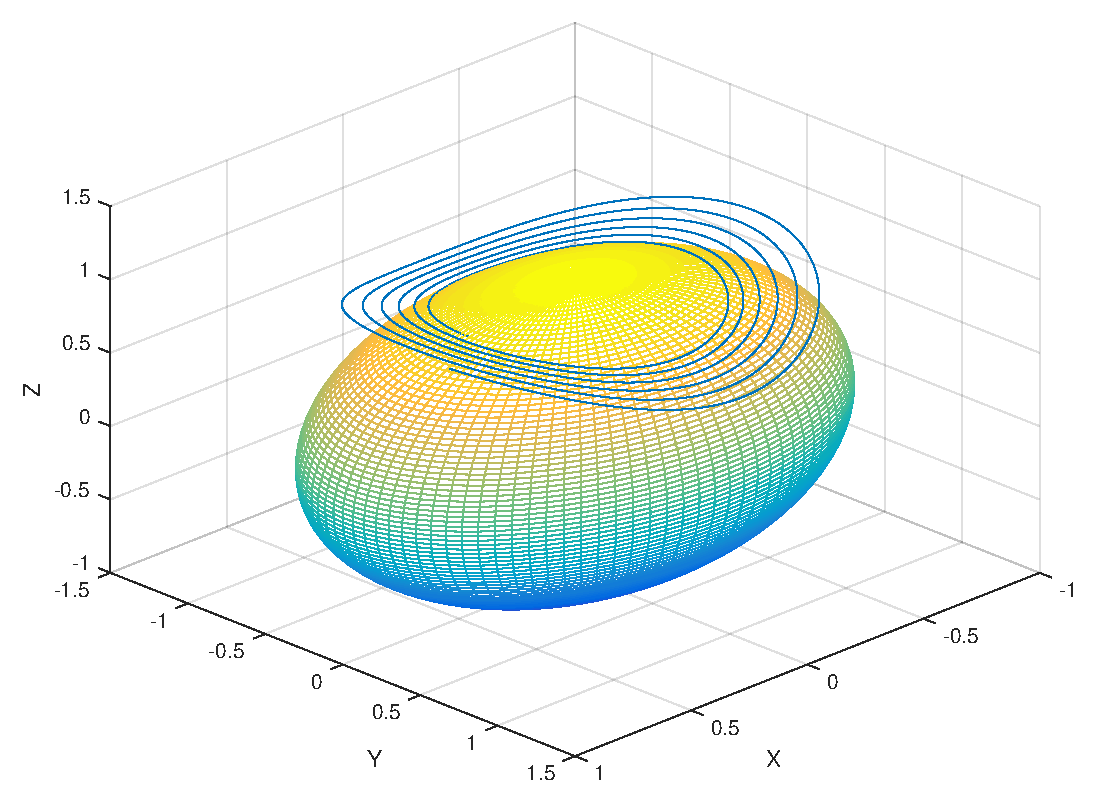
\includegraphics[width=0.6\textwidth]{03/explicit.pdf}
  \caption{非李群方法的数值结果}
  \label{fig:explicit}
\end{figure}

\begin{figure}[h!]
  \centering
  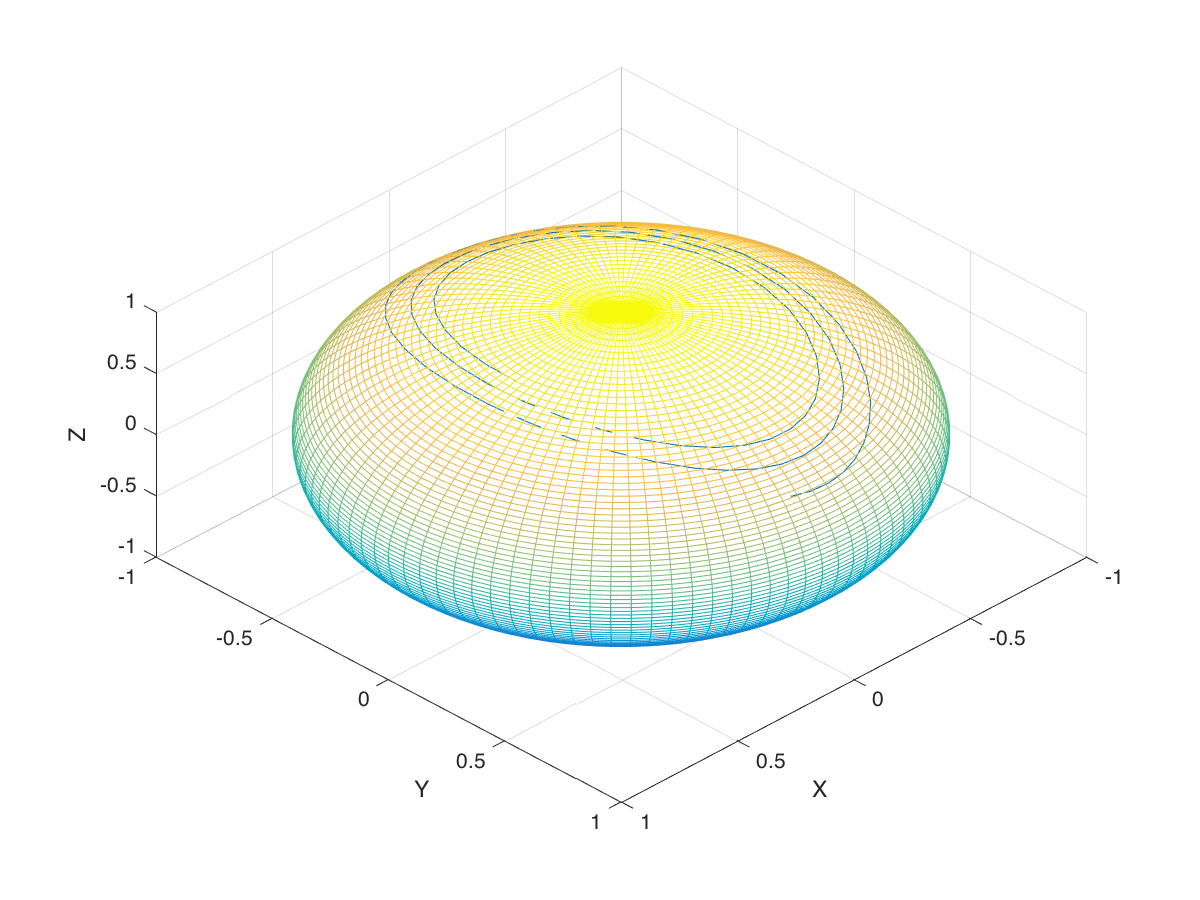
\includegraphics[width=0.6\textwidth]{03/cg2.png}
  \caption{李群方法的数值结果}
  \label{fig:midpoint}
\end{figure}

在本章,我们将用波形松弛方法 \cite{jiang2009wr} 来求解这个哈密尔顿系统 \eqref{eq:hal0}, 波形松弛方法的内容将在 \ref{sec:03wrintro} 中介绍.为了获得更好的数值效果,使用辛方法作为指导工具设计数值格式.

在这里,把结合了辛方法和波形松弛方法的方法叫做\textbf{辛波形松弛方法}.它是传统意义上的波形松弛方法的一个特例,将辛格式作为模型进行逼近,通过运用波形松弛方法解耦的特性,使计算过程更简单.波形松弛方法使问题求解相对隐式方法来说更加容易,同时,辛方法指导了波形松弛方法如何进行解耦.

在计算过程中,为了能更好地求解长时间区间的问题,引入窗口加速技术 \cite{jiang2006windowing,ladics2015error}. 窗口技术能够有效地减少波形松弛方法地迭代次数,同时能够保持辛方法的优秀特性.在 \cite{jiang2006windowing} 中作者给出了如何选取窗口长度,此外,窗口技术使得并行求解更加容易 \cite{liu2011waveform}.

接下来,对辛波形松弛方法做进一步地探讨和拓展.该拓展基于前面讨论的波形松弛方法对辛格式的改进,更进一步地研究了波形松弛数值格式在其他保持结构的问题里会有哪些实际可行的应用.对流形上的保结构的数值格式进行波形松弛方法地``改造'',以得到较为容易实现且速度较快的数值格式.

这里将给出求解流形上数值方法 RK-MK \cite{arieh2005liegroup} 方法的一个改进,该方法的``波形松弛化''再次说明了波形松弛方法在改造数值格式时的意义.这种改造一方面利用了波形松弛方法的解耦,迭代,实现简单等优点,另一方面还在通过迭代逼近数值格式,保持了原数值格式的优秀特性.

通常来说,我们的数值计算都是在一个空间上进行的,常用的空间是平直的线性欧氏空间.然而,某些方程具有特殊的意义,这些问题解地流存在在一个流形上.可是,在全空间上数值计算的误差存在会导致计算结果并不在该流形上.为了解决这一类问题,有一类流形上的李群方法被设计出来,这类方法能够很好地保证数值解落在流形上.上面提到的 RK-MK 算法就是这样一类方法.

然而,即使是李群方法,其数值结果会落到流形上,有些情况也并非令人满意,图 \ref{fig:rkmk2} 中的数值结果虽然保持在流形上了,但是并不是原问题应有的数值解,数值解只是误差出现在流形上了.
\begin{figure}[h!]
  \centering
  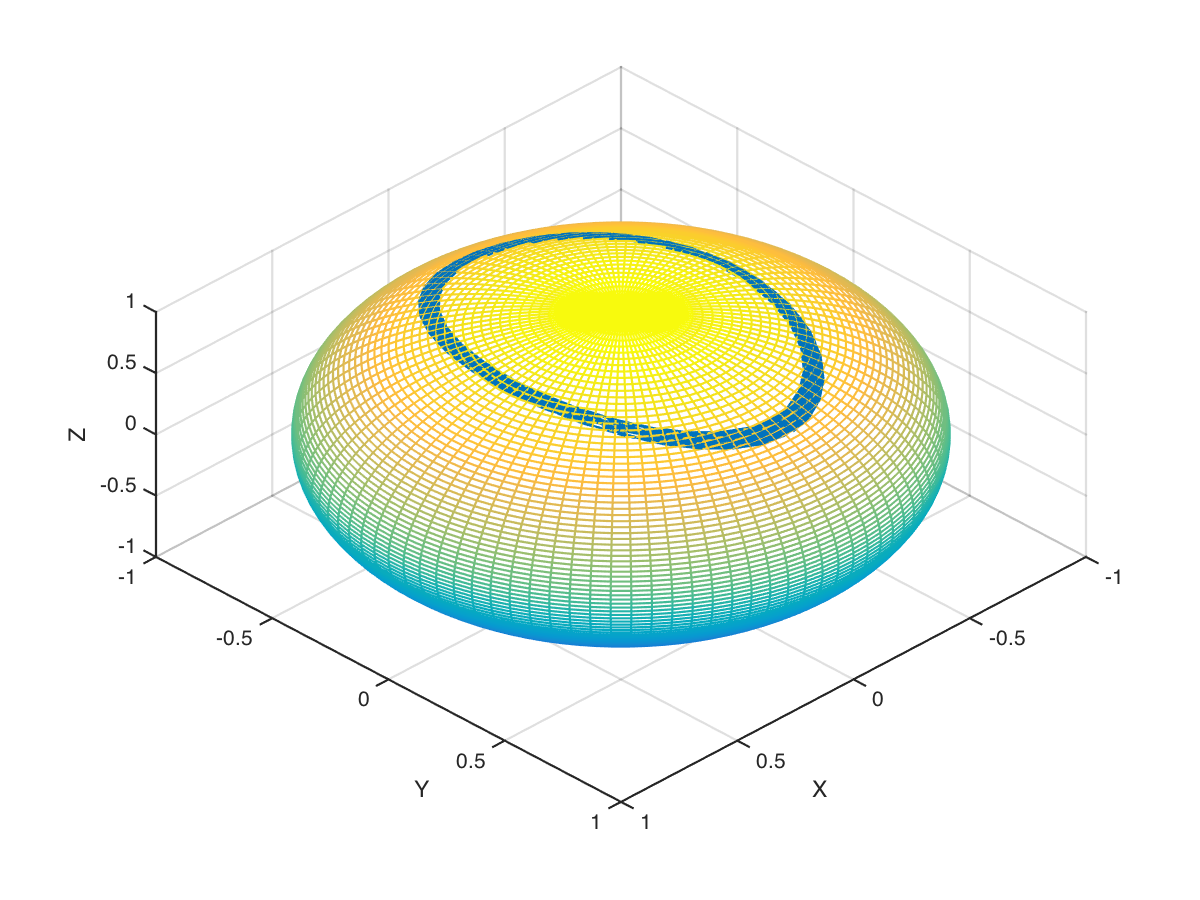
\includegraphics[width=0.6\textwidth]{03/rkmk2.png}
  \caption{较高阶李群方法的数值结果}
  \label{fig:rkmk2}
\end{figure}

事实上,根据哈密尔顿系统的理论,这种偏差可以由类似于辛方法的一类重要的李群方法来解决.根据辛积分理论,辛 Runge-Kutta 方法只有隐式的格式,这里可能需要隐式的 RK-MK 方法才能保持数值解在流形上保结构.

李群方法起初是由 Crouch 和 Grossman \cite{crouch1993numerical} 提出来的,即所谓的 Crouch-Grossman 方法,该方法得到了一系列地推广 \cite{faleinsen2001multi,zaletkin2010numerical,bulychev2001numerical,buono2003numerical,billo1992numerical}. 后来,在 1996 到 1999 年, Munthe-Kaas  等人提出了该方法的一个改进方法 \cite{mk1996lie,mk1997numerical,mk1998runge,mk1999high}, 即 MK-RK 方法,以及后面的一些推广 \cite{ostermann2010exponential,owren2000the,bruls2012lie,munthe2013onpost,garcla2011onalg}. Crouch-Grossman 方法和 MK-RK 方法都用到了李群的指数映射,联结了李群这个流形和李代数之间的关系,并且都利用了 Runge-Kutta 方法这种数值结构,使得阶数可以适当地提高,而且常规意义下的李群方法均为显式方法,计算较为简便.

我们要对隐式的 RK-MK 方法做出一些波形松弛类修正,使得数值方法能够具有较好的长时间稳定性,并且在计算上尽可能地简便,便于实现.该方法的思想来自于前半部分对辛方法的波形松弛类改进,和对 RK-MK 方法的理解.在计算过程中,不可避免地要引入窗口技术来加速.

本章的结构如下.在 \ref{sec:03wrintro} 中,对波形松弛方法进行简单介绍.在 \ref{sec:03wrhal} 中,分析了辛波形松弛方法,并给出了以下两个辛波形松弛方法的离散数值格式.同时,分析了系统哈密尔顿函数的守恒性,并介绍了窗口技术的选取问题.在 \ref{sec:04wrmani} 中,将对流形上的李群方法进行介绍,并且介绍 Crouch-Grossman 方法与 RK-MK 方法的相关理论,并陈述我们的修正算法.在 \ref{sec:03numerical} 中,给出了四个例子来说明问题.最后,在 \ref{sec:03conclusion} 中做了一个总结.

\section{波形松弛方法基本概念}\label{sec:03wrintro}
\esection{Introduction to the WR Method}

波形松弛方法来源于对大规模集成电路系统的研究 \cite{lelarasmee1982waveform}. 该方法分为两个部分,分裂和迭代.首先,需要使用分裂函数将大规模的系统划分为较小规模的子系统.接下来是迭代,迭代的过程先分别求解子系统,再在系统之间交换信息,进行下一次迭代,直到达到容许的误差.由此可见,波形松弛方法的显著特性是问题解耦和潜在的可并行性.

波形松弛方法是一种求解微分方程的迭代方式.它不是简简单单的通过求解离散过后的代数方程组的松弛方法,而是通过对方程分裂而构造出来的一种函数迭代方法,是``波形''的迭代.考虑如下的一阶常微分方程
\begin{equation}\label{eq:03ode}
\left\{
\begin{aligned}
\frac{dx(t)}{dt}&=f(x(t),t),\\
x(0)&=x_{0}.
\end{aligned}
\right.
\end{equation}

波形松弛方法的基本思想是找到一个分裂函数 $F(u,v,t)$ 满足 $F(u,u,t)=f(u,t)$, 分裂成如下方程
\begin{equation*}
\left\{
\begin{aligned}
\frac{dx^{k+1}(t)}{dt}&=F(x^{k+1}(t),x^{k}(t),t),\\
x^{k+1}(0)&=x_{0},
\end{aligned}
\right.
\end{equation*}
就能够快速求解并且更容易求解.不能逃避的一件事情是,在分裂函数 $F(u,v,t)$ 下,迭代后的函数序列 $x^{k}(t)$ 要收敛到原方程 \eqref{eq:03ode} 的解.

波形松弛方法的一个优点是能够把耦合的系统,通过分裂,在迭代过程中解耦为非耦合的系统,对于一些问题来讲,这为算法的并行计算提供了条件.同时,注意到,在计算的过程中,波形松弛方法能够将一些只能隐式格式求解的问题,化为显式或者半隐式的格式即可求解的问题.

一些常见的分裂函数取法有 Gauss-Jacobi 波形松弛方法, Gauss-Seidel 波形松弛方法,等等.作为一个例子,如果记 $u=(u_{1},u_{2},\ldots,u_{n})^{T}, v=(v_{1},v_{2},\ldots,v_{n})^{T}$, 并且方程的形式为
\begin{equation*}
\left\{
\begin{aligned}
\frac{dx_{1}(t)}{dt}&=f_{1}(x_{1}(t),x_{2}(t),\ldots,x_{n}(t),t),\\
\frac{dx_{2}(t)}{dt}&=f_{2}(x_{1}(t),x_{2}(t),\ldots,x_{n}(t),t),\\
\ldots&\ldots\ldots\ldots\ldots\ldots\ldots\\
\frac{dx_{n}(t)}{dt}&=f_{n}(x_{1}(t),x_{2}(t),\ldots,x_{n}(t),t),\\
x_{1}(0)&=x_{1,0},x_{2}(0)=x_{2,0},\ldots,x_{n}(0)=x_{n,0},
\end{aligned}
\right.
\end{equation*}
Gauss-Jacobi 波形松弛方法和 Gauss-Seidel 波形松弛方法的分裂函数分别为
\begin{align}\label{eq:wr}
&F_{i}(u,v,t)=f_{i}(v_{1},v_{2},\ldots,v_{i-1},u_{i},v_{i+1},\ldots,v_{n},t)\quad \text{(Gauss-Jacobi~WR)},\\
&F_{i}(u,v,t)=f_{i}(u_{1},u_{2},\ldots,u_{i-1},u_{i},v_{i+1},\ldots,v_{n},t)\quad \text{(Gauss-Seidel~WR)}.
\end{align}

简而言之,波形松弛方法 \cite{jiang2009wr} 作为一个数学工具,思想起源于大规模集成电路的求解.当系统的规模大到一定程度的时候,使用现有的计算资源求解该问题就变得困难,可以把大型的系统分裂成更易于求解的小型系统来计算.为了达到这个目标,选取分裂函数 $F(z,y)$ 使得 $F(z,z)=f(z)$, 然后将方程 \eqref{eq:hal0} 中的 $f(z)$ 替换为 $F(z,y)$. 接下来为每一个子系统选择一个合适的初始迭代,将 $F(z,y)$ 中的 $y$ 作为已知函数, $z$ 作为未知函数,这样每次迭代的计算量就降低了.然而,由于初值的选取和格式的设计,这样的一步计算不会得到系统的真实解,还要通过迭代来保证收敛到方程的真解.通常将迭代方程记作 $\dot{z}^{k+1}=F(z^{k+1},z^{k})$, 其中 $k=0,1,\cdots$ 是迭代次数.


\section{哈密尔顿系统的辛波形松弛方法}\label{sec:03wrhal}
\esection{Symplectic WR Methods for Hamiltonian Systems}
在本小节,我们分析哈密尔顿系统 \eqref{eq:hal0} 的辛波形松弛方法.把方程 \eqref{eq:hal0} 写成如下形式
\begin{equation}\label{eq:hal1}
\dot{z}=f(z),
\end{equation}
式中 $z=(q;p)$ 为区间 $[0,T]$ 上的未知函数, $f(z)$ 是方程 \eqref{eq:hal0} 右端函数.

对于波形松弛方法,取一个分裂函数 $F(x,y)$ 使得 $F(z,z)=f(z)$. 该分裂函数用于对系统 \eqref{eq:hal1} 进行解耦.对波形松弛方法,有如下已知的结果.

\begin{theorem}[ODE 的波形松弛方法 \cite{jiang2009wr}]\label{thm:wr}
	\emph{如果 \eqref{eq:hal1} 的分裂函数 $F(x,y)$ 对变量 $x$ 和 $y$ 是 Lipschitz 连续的,那么波形松弛方法收敛.}
\end{theorem}

\subsection{连续时间的辛波形松弛方法}
\esubsection{The Continuous-time Symplectic WR Method}
辛波形松弛方法属于传统波形松弛方法的特例,所以定理 \ref{thm:wr} 自动成立.接下来,我们进一步研究哈密尔顿函数 $H$ 的变化情况.

\begin{theorem}
\emph{如果辛波形松弛方法收敛,并且 \eqref{eq:hal1} 里的右端函数 $f$ 有界,则哈密尔顿函数收敛到常函数.}
\end{theorem}

{\textbf{证明}} 记 $H_0$ 为系统的哈密尔顿函数.因为该哈密尔顿函数 $H_0$ 为常函数,有
\begin{equation*}
\frac{dH_0}{dt}=0.
\end{equation*}
记 $H^{k+1}$ 为第 $k+1$ 此迭代的哈密尔顿函数,即
\begin{equation*}
H^{k+1}=H(q^{k+1},p^{k+1}),
\end{equation*}
式中 $q^{k+1}$ 和 $p^{k+1}$ 为第 $k+1$ 步的位移和动量函数.

接下来,来看函数 $H^{k+1}-H_0$ 的导数.
\begin{equation*}
\begin{aligned}
\frac{d(H^{k+1}-H_0)}{dt}=&H_q(z^{k+1})^TF_1(z^{k+1},z^{k})-H_q(z)^TF_1(z,z)\\
&+H_p(z^{k+1})^TF_2(z^{k+1},z^{k})-H_p(z)^TF_2(z,z),
\end{aligned}
\end{equation*}
式中 $F_1$ 和 $F_2$ 分别是 $H_p$ 和 $-H_q$ 的分裂函数.

于是,有
\begin{equation*}
\begin{aligned}
\|H_q(z^{k+1})^TF_1(z^{k+1},z^{k})&-H_q(z)^TF_1(z,z)\|\\
&=\|H_q(z^{k+1})^TF_1(z^{k+1},z^{k})-H_q(z)^TF_1(z^{k+1},z^{k})\\
&+H_q(z)^TF_1(z^{k+1},z^{k})-H_q(z)^TF_1(z,z^{k})\\
&+H_q(z)^TF_1(z,z^{k})-H_q(z)^TF_1(z,z)\|\\
&\le\|H_q(z^{k+1})^TF_1(z^{k+1},z^{k})-H_q(z)^TF_1(z^{k+1},z^{k})\|\\
&+\|H_q(z)^TF_1(z^{k+1},z^{k})-H_q(z)^TF_1(z,z^{k})\|\\
&+\|H_q(z)^TF_1(z,z^{k})-H_q(z)^TF_1(z,z)\|\\
&\le A_1\|z^{k+1}-z\|+B_1\|z^{k}-z\|,
\end{aligned}
\end{equation*}
式中 $A_1$ 和 $B_1$ 是常数.

类似地,有
\begin{equation*}
\|H_q(z^{k+1})^TF_1(z^{k+1},z^{k})-H_q(z)^TF_1(z,z)\|\le A_2\|z^{k+1}-z\|+B_2\|z^{k}-z\|,
\end{equation*}
式中 $A_2$ 和 $B_2$ 是常数.

因此
\begin{equation*}
\left\|\frac{dH^{k+1}-H_0}{dt}\right\|\le (A_1+A_2)\|z^{k+1}-z\|+(B_1+B_2)\|z^{k}-z\| \to 0.
\end{equation*}

上面最后一个式子成立是因为波形松弛方法的收敛性.注意到 $H^{k+1}(z(0))=H_0(z(0))$, 定理即可获得证明.

证毕.

\subsection{离散时间的辛波形松弛方法}
\esubsection{The Discrete-time Symplectic WR Method}
离散的数值格式并不能够很直接地看出来.为了构造离散格式,必须同时兼顾辛格式和分裂函数.假设一个单步的辛格式为
\begin{equation*}
z_{n+1}=z_{n}+h g(z_{n+1},z_{n}),
\end{equation*}
其相应的辛波形松弛方法即为
\begin{equation}\label{eq:discrete}
z_{n+1}^{k+1}=z_{n}^{k+1}+h \tilde{F}(z_{n+1}^{k+1},z_{n+1}^{k},z_{n}^{k+1},z_{n}^{k}),
\end{equation}
式中满足 $\tilde{F}(x,y,x,y)=F(x,y)$ 和 $\tilde{F}(x,x,y,y)=g(x,y)$.

\begin{theorem}
\emph{如果辛波形松弛方法收敛,并且辛格式对变量 $z_{n}$ 和 $z_{n+1}$ Lipschitz 连续,那么辛波形松弛方法的哈密尔顿函数收敛到离散格式的哈密尔顿函数.}
\end{theorem}

{\textbf{证明}} 记 $H^{k+1}_{n+1}$ 为 $H(z_{n+1}^{k+1})$, $H_{n+1}$ 为 $H(z_{n+1})$ 其中 $z_{n+1}^{k+1}$ 和 $z_{n+1}$ 分别为辛波形松弛方法和辛方法的数值解.

我们说离散的辛波形松弛方法是收敛的,如果满足 $\|z_{n+1}^{k+1} - z_{n+1}\| \to 0~(k \to \infty)$.

注意到
\begin{equation*}
\begin{aligned}
\|H^{k+1}_{n+1}-H_{n+1}\|&=\|H(z_{n}^{k+1}+h \tilde{F}(z_{n+1}^{k+1},z_{n+1}^{k},z_{n}^{k+1},z_{n}^{k}))-H(z_{n+1})\|\\
&\le \|\tilde{H}(z_{n+1}^{k+1},z_{n+1}^{k},z_{n}^{k+1},z_{n}^{k})-\tilde{H}(z_{n+1},z_{n+1}^{k},z_{n}^{k+1},z_{n}^{k})\|\\
&+\|\tilde{H}(z_{n+1},z_{n+1}^{k},z_{n}^{k+1},z_{n}^{k})-\tilde{H}(z_{n+1},z_{n+1},z_{n}^{k+1},z_{n}^{k})\|\\
&+\|\tilde{H}(z_{n+1},z_{n+1},z_{n}^{k+1},z_{n}^{k})-\tilde{H}(z_{n+1},z_{n+1},z_{n},z_{n}^{k})\|\\
&+\|\tilde{H}(z_{n+1},z_{n+1},z_{n},z_{n}^{k})-\tilde{H}(z_{n+1},z_{n+1},z_{n},z_{n})\|\\
&+\|\tilde{H}(z_{n+1},z_{n+1},z_{n},z_{n})-H(z_{n+1})\|,\\
\end{aligned}
\end{equation*}
式中 $\tilde{H}(x,y,z,w)=z+h \tilde{F}(x,y,z,w)$ 为数值辛格式,所以有
\begin{equation*}
\tilde{H}(z_{n+1},z_{n+1},z_{n},z_{n})=H(z_{n+1}).
\end{equation*}

因此,有
\begin{equation*}
\|H^{k+1}_{n+1}-H_{n+1}\|\le C(\|z_{n+1}^{k+1}-z_{n+1}\|+ \|z_{n+1}^{k}-z_{n+1}\|+ \|z_{n}^{k+1}-z_{n}\|+ \|z_{n}^{k}-z_{n}\|),
\end{equation*}
式中 $C$ 为常数.上面的不等式表明 $\|H^{k+1}_{n+1}-H_{n+1}\| \to 0$ 随着 $k \to \infty$.

证毕.

针对辛波形松弛方法,在这里给出两种重要的例子说明分裂函数的选取方法.

\subsubsection{辛欧拉波形松弛方法}
\esubsubsection{Symplectic Euler Waveform Relaxation Method}
对于哈密尔顿函数 \eqref{eq:hal0} 和辛欧拉方法 \cite{hairer2014challenges}
\begin{equation}\label{eq:symeuler1}
  \begin{array}{c}
    q_{n+1}=q_{n}+hH_{p}(q_{n},p_{n+1}),\\
    p_{n+1}=p_{n}-hH_{q}(q_{n},p_{n+1}).
  \end{array}
\end{equation}

将 Jacobi 波形松弛方法作为分裂函数,有
\begin{equation*}
  \left\{
    \begin{aligned}
      q_{1,n+1}^{(k+1)}&=q_{1,n}^{(k+1)}+hH_{p_{1}}(q_{1,n}^{(k+1)},q_{2,n}^{(k)},\ldots,q_{d,n}^{(k)},p_{1,n+1}^{(k)},p_{2,n+1}^{(k)},\ldots,p_{d,n+1}^{(k)}),\\
      q_{2,n+1}^{(k+1)}&=q_{2,n}^{(k+1)}+hH_{p_{2}}(q_{1,n}^{(k)},q_{2,n}^{(k+1)},\ldots,q_{d,n}^{(k)},p_{1,n+1}^{(k)},p_{2,n+1}^{(k)},\ldots,p_{d,n+1}^{(k)}),\\
      \ldots&\ldots\ldots\ldots\ldots\ldots\ldots\\
      q_{d,n+1}^{(k+1)}&=q_{d,n}^{(k+1)}+hH_{p_{d}}(q_{1,n}^{(k)},q_{2,n}^{(k)},\ldots,q_{d,n}^{(k+1)},p_{1,n+1}^{(k)},p_{2,n+1}^{(k)},\ldots,p_{d,n+1}^{(k)}),\\
      p_{1,n+1}^{(k+1)}&=p_{1,n}^{(k+1)}-hH_{q_{1}}(q_{1,n}^{(k)},q_{2,n}^{(k)},\ldots,q_{d,n}^{(k)},p_{1,n+1}^{(k+1)},p_{2,n+1}^{(k)},\ldots,p_{d,n+1}^{(k)}),\\
      p_{2,n+1}^{(k+1)}&=p_{2,n}^{(k+1)}-hH_{q_{2}}(q_{1,n}^{(k)},q_{2,n}^{(k)},\ldots,q_{d,n}^{(k)},p_{1,n+1}^{(k)},p_{2,n+1}^{(k+1)},\ldots,p_{d,n+1}^{(k)}),\\
      \ldots&\ldots\ldots\ldots\ldots\ldots\ldots\\
      p_{d,n+1}^{(k+1)}&=p_{d,n}^{(k+1)}-hH_{q_{d}}(q_{1,n}^{(k)},q_{2,n}^{(k)},\ldots,q_{d,n}^{(k)},p_{1,n+1}^{(k)},p_{2,n+1}^{(k)},\ldots,p_{d,n+1}^{(k+1)}).\\
    \end{aligned}
  \right.
\end{equation*}
如果 $p,q \in \mathbb{R}$, 那么上面的方法化为
\begin{equation}\label{eq:schemejacobi}
  \begin{aligned}
    q_{n+1}^{(k+1)}&=q_{n}^{(k+1)}+hH_{p}(q_{n}^{(k+1)},p_{n+1}^{(k)}),\\
    p_{n+1}^{(k+1)}&=p_{n}^{(k+1)}-hH_{q}(q_{n}^{(k)},p_{n+1}^{(k+1)}).
  \end{aligned}
\end{equation}
类似地,使用 Gauss-Seidel WR 波形松弛方法作为分裂函数,有
\begin{equation*}
  \left\{
    \begin{aligned}
      q_{1,n+1}^{(k+1)}&=q_{1,n}^{(k+1)}+hH_{p_{1}}(q_{1,n}^{(k+1)},q_{2,n}^{(k)},\ldots,q_{d,n}^{(k)},p_{1,n+1}^{(k)},p_{2,n+1}^{(k)},\ldots,p_{d,n+1}^{(k)}),\\
      q_{2,n+1}^{(k+1)}&=q_{2,n}^{(k+1)}+hH_{p_{2}}(q_{1,n}^{(k+1)},q_{2,n}^{(k+1)},\ldots,q_{d,n}^{(k)},p_{1,n+1}^{(k)},p_{2,n+1}^{(k)},\ldots,p_{d,n+1}^{(k)}),\\
      \ldots&\ldots\ldots\ldots\ldots\ldots\ldots\\
      q_{d,n+1}^{(k+1)}&=q_{d,n}^{(k+1)}+hH_{p_{d}}(q_{1,n}^{(k+1)},q_{2,n}^{(k+1)},\ldots,q_{d,n}^{(k+1)},p_{1,n+1}^{(k)},p_{2,n+1}^{(k)},\ldots,p_{d,n+1}^{(k)}),\\
      p_{1,n+1}^{(k+1)}&=p_{1,n}^{(k+1)}-hH_{q_{1}}(q_{1,n}^{(k+1)},q_{2,n}^{(k+1)},\ldots,q_{d,n}^{(k+1)},p_{1,n+1}^{(k+1)},p_{2,n+1}^{(k)},\ldots,p_{d,n+1}^{(k)}),\\
      p_{2,n+1}^{(k+1)}&=p_{2,n}^{(k+1)}-hH_{q_{2}}(q_{1,n}^{(k+1)},q_{2,n}^{(k+1)},\ldots,q_{d,n}^{(k+1)},p_{1,n+1}^{(k+1)},p_{2,n+1}^{(k+1)},\ldots,p_{d,n+1}^{(k)}),\\
      \ldots&\ldots\ldots\ldots\ldots\ldots\ldots\\
      p_{d,n+1}^{(k+1)}&=p_{d,n}^{(k+1)}-hH_{q_{d}}(q_{1,n}^{(k+1)},q_{2,n}^{(k+1)},\ldots,q_{d,n}^{(k+1)},p_{1,n+1}^{(k+1)},p_{2,n+1}^{(k+1)},\ldots,p_{d,n+1}^{(k+1)}).
    \end{aligned}
  \right.
\end{equation*}
如果 $p,q \in \mathbb{R}$, 则上面的方法化为
\begin{equation}\label{eq:schemegauss}
  \begin{aligned}
    q_{n+1}^{(k+1)}&=q_{n}^{(k+1)}+hH_{p}(q_{n}^{(k+1)},p_{n+1}^{(k)}),\\
    p_{n+1}^{(k+1)}&=p_{n}^{(k+1)}-hH_{q}(q_{n}^{(k+1)},p_{n+1}^{(k+1)}).
  \end{aligned}
\end{equation}

从形式上来看,如果忽略下角标 $p$ 和 $q$, 这个格式可以看成波形松弛方法,如果忽略上角标则可以看成是辛欧拉方法.

\subsubsection{辛 Runge-Kutta 波形松弛方法}
\esubsubsection{The Symplectic Runge-Kutta WR Method}
对于 Runge-Kutta 方法,使用了一个将 Runge-Kutta 方法和波形松弛方法结合的策略 \cite{bellen1993use,bellen1994contractivity}. 可以知道, $\nu$ 步的 Runge-Kutta 方法可以写成
\begin{equation*}
  \left\lbrace
    \begin{aligned}
      Y_{n+1}^{r}&=\eta(t_{n})+h\sum_{s=1}^{\nu}a_{rs}f(t_{n+1}^{s},Y_{n+1}^{s}),\quad r=1,\cdots, \nu, \\
      \eta(t_{n+1})&=\eta(t_{n})+h\sum_{s=1}^{\nu}b_{s}f(t_{n+1}^{s},Y_{n+1}^{s}).
    \end{aligned}
  \right.
\end{equation*}

其对应的 Butcher 表可以写成

\begin{center}
  \begin{tabular}{c|cccc}
    $c_1$&$a_{11}$&$a_{12}$&$\cdots$&$a_{1\nu}$\\
    $c_2$&$a_{21}$&$a_{22}$&$\cdots$&$a_{2\nu}$\\
    $\vdots$&$\vdots$&$\vdots$&$\ddots$&$\vdots$\\
    $c_{\nu}$&$a_{\nu 1}$&$a_{\nu 2}$&$\cdots$&$a_{\nu \nu}$\\
    \hline
         &$b_{1}$&$b_{2}$&$\cdots$&$b_{\nu}$
  \end{tabular}
\end{center}

如果该 Runge-Kutta 的 Butcher 表满足
\begin{equation*}
  b_ia_{ij}+b_ja_{ji}=b_ib_j,\quad \textrm{对所有}\,\, i,j=1,2,\cdots,\nu,
\end{equation*}
则该 Runge-Kutta 方法是保辛的.

这里,采用如下的辛波形松弛方法 \cite{bellen1993use}
\begin{equation*}
  \left\lbrace
    \begin{aligned}
      Y_{n+1}^{r,(k+1)}&=\eta^{(k+1)}(t_{n})+h\sum_{s=1}^{\nu}a_{rs}F(t_{n+1}^{s},Y_{n+1}^{s,(k+1)},Y_{n+1}^{s,(k)}),\quad r=1,\cdots, \nu, \\
      \eta^{(k+1)}(t_{n+1})&=\eta^{(k+1)}(t_{n})+h\sum_{s=1}^{\nu}b_{s}F(t_{n+1}^{s},Y_{n+1}^{s,(k+1)},Y_{n+1}^{s,(k)}).
    \end{aligned}
  \right.
\end{equation*}

根据构造辛波形松弛方法的策略,可以将 Gauss-Jacobi~波形松弛方法 (WRGJ),和 Gauss-Seidel~波形松弛方法(WRGS) 应用于 Runge-Kutta方法,得到相应的 WRGJRK 和 WRGSRK 方法.

WRGJRK 方法为, 对于 $i=1,\cdots,2d$
\begin{equation*}
  \left\lbrace
    \begin{aligned}
      Y_{r,i}^{(k+1)}=&\eta_{i}^{(k+1)}(t_{n})+h\sum_{s=1}^{\nu}a_{rs}f_i(t_{n+1}^{s},Y_{s,1}^{(k)},\cdots,\\
      &Y_{s,i-1}^{(k)},Y_{s,i}^{(k+1)},Y_{s,i+1}^{(k)},\cdots,Y_{s,2d}^{(k)}),\quad r=1,\cdots, \nu, \\
      \eta_{i}^{(k+1)}(t_{n+1})=&\eta_{i}^{(k+1)}(t_{n})+h\sum_{s=1}^{\nu}b_{s}f_i(t_{n+1}^{s},Y_{s,1}^{(k)},\cdots,\\
      &Y_{s,i-1}^{(k)},Y_{s,i}^{(k+1)},Y_{s,i+1}^{(k)},\cdots,Y_{s,2d}^{(k)}).
    \end{aligned}
  \right.
\end{equation*}

WRGSRK 方法为, 对于 $i=1,\cdots,2d$
\begin{equation*}
  \left\lbrace
    \begin{aligned}
      Y_{r,i}^{(k+1)}=&\eta_{i}^{(k+1)}(t_{n})+h\sum_{s=1}^{\nu}a_{rs}f_i(t_{n+1}^{s},Y_{s,1}^{(k+1)},\cdots,\\
      &Y_{s,i-1}^{(k+1)},Y_{s,i}^{(k+1)},Y_{s,i+1}^{(k)},\cdots,Y_{s,2d}^{(k)}),\quad r=1,\cdots, \nu, \\
      \eta_{i}^{(k+1)}(t_{n+1})=&\eta_{i}^{(k+1)}(t_{n})+h\sum_{s=1}^{\nu}b_{s}f_i(t_{n+1}^{s},Y_{s,1}^{(k+1)},\cdots,\\
      &Y_{s,i-1}^{(k+1)},Y_{s,i}^{(k+1)},Y_{s,i+1}^{(k)},\cdots,Y_{s,2d}^{(k)}).
    \end{aligned}
  \right.
\end{equation*}

把这些方法作用于哈密尔顿系统,有如下的 WRGJRK 格式, 对于 $i=1,\cdots,d$, $r=1,\cdots,\nu$
\begin{equation}\label{eq:schemerkjacobi}
  \left\lbrace
    \begin{aligned}
      Q_{r,i}^{(k+1)}&=q_{i}^{(k+1)}(t_{n})+h\sum_{s=1}^{\nu}a_{rs}H_{p,i}(Q_{s,1}^{(k)},\cdots,Q_{s,i-1}^{(k)},\\
                            &Q_{s,i}^{(k+1)},Q_{s,i+1}^{(k)},\cdots,Q_{s,d}^{(k)},P_{s,1}^{(k)},\cdots,P_{s,d}^{(k)}),\\
      P_{r,i}^{(k+1)}&=p_{i}^{(k+1)}(t_{n})-h\sum_{s=1}^{\nu}a_{rs}H_{q,i}(Q_{s,1}^{(k)},\cdots,Q_{s,d}^{(k)},\\
                            &P_{s,1}^{(k)},\cdots,P_{s,i-1}^{(k)},P_{s,i}^{(k+1)},P_{s,i+1}^{(k)}\cdots,P_{s,d}^{(k)}),\\
      q_{i}^{(k+1)}(t_{n+1})&=q_{i}^{(k+1)}(t_{n})+h\sum_{s=1}^{\nu}b_{s}H_{p,i}(Q_{s,1}^{(k)},\cdots,Q_{s,i-1}^{(k)},\\
                            &Q_{s,i}^{(k+1)},Q_{s,i+1}^{(k)},\cdots,Q_{s,d}^{(k)},P_{s,1}^{(k)},\cdots,P_{s,d}^{(k)}),\\
      p_{i}^{(k+1)}(t_{n+1})&=p_{i}^{(k+1)}(t_{n})-h\sum_{s=1}^{\nu}b_{s}H_{q,i}(Q_{s,1}^{(k)},\cdots,Q_{s,d}^{(k)},\\
                            &P_{s,1}^{(k)},\cdots,P_{s,i-1}^{(k)},P_{s,i}^{(k+1)},P_{s,i+1}^{(k)}\cdots,P_{s,d}^{(k)}),\\
    \end{aligned}
  \right.
\end{equation}

和 WRGSRK 格式, 对于 $i=1,\cdots,d$, $r=1,\cdots,\nu$
\begin{equation*}
  \left\lbrace
    \begin{aligned}
      Q_{r,i}^{(k+1)}&=q_{i}^{(k+1)}(t_{n})+h\sum_{s=1}^{\nu}a_{rs}H_{p,i}(Q_{s,1}^{(k+1)},\cdots,Q_{s,i-1}^{(k+1)},\\
                            &Q_{s,i}^{(k+1)},Q_{s,i+1}^{(k)},\cdots,Q_{s,d}^{(k)},P_{s,1}^{(k)},\cdots,P_{s,d}^{(k)}),\\
      P_{r,i}^{(k+1)}&=p_{i}^{(k+1)}(t_{n})-h\sum_{s=1}^{\nu}a_{rs}H_{q,i}(Q_{s,1}^{(k+1)},\cdots,Q_{s,d}^{(k+1)},\\
                            &P_{s,1}^{(k+1)},\cdots,P_{s,i-1}^{(k+1)},P_{s,i}^{(k+1)},P_{s,i+1}^{(k)}\cdots,P_{s,d}^{(k)}),\\
      q_{i}^{(k+1)}(t_{n+1})&=q_{i}^{(k+1)}(t_{n})+h\sum_{s=1}^{\nu}b_{s}H_{p,i}(Q_{s,1}^{(k+1)},\cdots,Q_{s,i-1}^{(k+1)},\\
                            &Q_{s,i}^{(k+1)},Q_{s,i+1}^{(k)},\cdots,Q_{s,d}^{(k)},P_{s,1}^{(k)},\cdots,P_{s,d}^{(k)}),\\
      p_{i}^{(k+1)}(t_{n+1})&=p_{i}^{(k+1)}(t_{n})-h\sum_{s=1}^{\nu}b_{s}H_{q,i}(Q_{s,1}^{(k+1)},\cdots,Q_{s,d}^{(k+1)},\\
                            &P_{s,1}^{(k+1)},\cdots,P_{s,i-1}^{(k+1)},P_{s,i}^{(k+1)},P_{s,i+1}^{(k)}\cdots,P_{s,d}^{(k)}).\\
    \end{aligned}
  \right.
\end{equation*}

\subsection{离散时间的辛波形松弛方法的进一步讨论}
\esubsection{Further Discussions on the Discrete-time Symplectic WR Method}
接下来,对格式 \eqref{eq:schemejacobi} 做出简要分析.格式 \eqref{eq:schemegauss} 可以给出类似的结果.

对于波形松弛方法来说,需要给出一个初始猜测 $q_{i}^{(0)},~p_{i}^{(0)}~\text{for}~i=0,1,\ldots,N$, 其中 $i$ 是时间网格的指标.选定了初始迭代之后,就得到了如下的波形松弛格式的算法.通常来说,初始迭代可以取作 $q_{i}^{(0)}=q_{0},~p_{i}^{(0)}=p_{0}.$

\begin{algorithm}
\caption{辛欧拉波形松弛方法}
\label{alg:alg1}
\begin{algorithmic}
    \STATE 设置初始迭代值 $q_{i}^{(0)}, p_{i}^{(0)} \text{for}~i=0,1,\ldots,N.$
    \WHILE{达到容许的误差}
        \STATE 使用数值格式 \eqref{eq:schemejacobi}, 用 $q^{(k)},~p^{(k)}$ 求解 $q^{(k+1)},~p^{(k+1)}$.
    \ENDWHILE
\end{algorithmic}
\end{algorithm}


\begin{theorem}[算法 \eqref{alg:alg1} 的收敛性]\label{thm:sj}\\
\emph{如果 $H_{p}$ 和 $H_{q}$ 对变量 $p$ 和 $q$ Lipschitz 连续,即,
\begin{equation*}
  \begin{aligned}
    \|H_{p}(q_{1},p)-H_{p}(q_{2},p)\| &\le M_{q} \|q_{1}-q_{2}\|, \\
    \|H_{p}(q,p_{1})-H_{p}(q,p_{2})\| &\le M_{p} \|p_{1}-p_{2}\|, \\
    \|H_{q}(q_{1},p)-H_{q}(q_{2},p)\| &\le L_{q} \|q_{1}-q_{2}\|, \\
    \|H_{q}(q,p_{1})-H_{q}(q,p_{2})\| &\le L_{p} \|p_{1}-p_{2}\|, \\
  \end{aligned}
\end{equation*}
那么格式 \eqref{eq:schemejacobi} 收敛.}
\end{theorem}

{\textbf{证明}} 记 $\epsilon_{q,n}^{(k)}=q_{n}^{(k)}-q_{n}$ 和 $\epsilon_{p,n}^{(k)}=p_{n}^{(k)}-p_{n}$, 然后将式 \eqref{eq:schemejacobi} 和 \eqref{eq:symeuler1} 相减,得到
  \begin{equation*}
    \begin{aligned}
      \epsilon_{q,n+1}^{(k+1)}&=\epsilon_{q,n}^{(k+1)}+h(H_{p}(q_{n}^{(k+1)},p_{n+1}^{(k)})-H_{p}(q_{n},p_{n+1})),\\
      \epsilon_{p,n+1}^{(k+1)}&=\epsilon_{p,n}^{(k+1)}-h(H_{q}(q_{n}^{(k)},p_{n+1}^{(k+1)})-H_{q}(q_{n},p_{n+1})).
    \end{aligned}
  \end{equation*}
  然后,记 $e_{p,n}^{k}=\|\epsilon_{p,n}^{(k)}\|$, 然后应用 Lipschitz 条件,有
  \begin{equation*}
    \begin{aligned}
      e_{q,n+1}^{k+1}&\le e_{q,n}^{k+1}+hM_{q}e_{q,n}^{k+1}+hM_{p}e_{p,n+1}^{k},\\
      e_{p,n+1}^{k+1}&\le e_{p,n}^{k+1}+hL_{q}e_{q,n}^{k}+hL_{p}e_{p,n+1}^{k+1}.
    \end{aligned}
  \end{equation*}
  令 $\alpha=\frac{1}{1-hL_{p}}$, $\beta=\frac{hL_{q}}{1-hL_{p}}$, $\gamma=1+hM_{q}$ 和 $\theta=hM_{p}$, 有
  \begin{equation*}
    \begin{aligned}
      e_{q,n+1}^{k+1}&\le \gamma e_{q,n}^{k+1}+\theta e_{p,n+1}^{k},\\
      e_{p,n+1}^{k+1}&\le \alpha e_{p,n}^{k+1}+\beta e_{q,n}^{k}.
    \end{aligned}
  \end{equation*}
  注意到 $e_{q,0}^{k}=0, e_{p,0}^{k}=0$, 能够得到
  \begin{equation*}
    \begin{aligned}
      e_{q,n+1}^{k+1}&\le \gamma^{n}\theta e_{p,1}^{k}+\gamma^{n-1}\theta e_{p,2}^{k}+\ldots+\gamma \theta e_{p,n}^{k}+\theta e_{p,n+1}^{k},\\
      e_{p,n+1}^{k+1}&\le \alpha^{n-1}\beta e_{q,1}^{k}+\alpha^{n-2}\beta e_{q,2}^{k}+\ldots+\alpha \beta
      e_{q,n-1}^{k}+\beta e_{q,n}^{k}.
    \end{aligned}
  \end{equation*}
  为了记号简单,把上面的不等式写作
  \begin{equation*}
    \begin{aligned}
      e_{q,n+1}^{k+1}&\le \sum_{a+b=n+1}\gamma^{a}\theta e_{p,b}^{k},\\
      e_{p,n+1}^{k+1}&\le \sum_{a+b=n}\alpha^{a}\beta e_{q,b}^{k}.
    \end{aligned}
  \end{equation*}
  然后得到
  \begin{equation*}
    \begin{aligned}
      e_{q,n+1}^{k+1}&\le \beta\theta \sum_{a+b+c=n}\alpha^{a}\gamma^{b} e_{q,c}^{k-1},\\
      e_{p,n+1}^{k+1}&\le \beta \theta \sum_{a+b+c=n}\alpha^{a}\gamma^{b} e_{p,c}^{k-1}.
    \end{aligned}
  \end{equation*}
  上面的两个不等式有相同的形式,所以将其记作
  \begin{equation*}
    e_{n+1}^{k+1}\le \beta \theta \sum_{a+b+c=n}\alpha^{a}\gamma^{b} e_{c}^{k-1},
  \end{equation*}
  式中 $e_{n+1}^{k+1}$ 代表 $e_{p,n+1}^{k+1}$ 或 $e_{q,n+1}^{k+1}$. 如果 $k+1=2t$, 那么有
  \begin{equation*}
    e_{n+1}^{k+1}\le \beta^{t} \theta^{t} \sum_{a+b+c=n-t+1}\alpha^{a}\gamma^{b} e_{c}^{0}.
  \end{equation*}
  由于 $c\le n-t+1$, $e_{n+1}^{k+1}$ 随着 $t$ 的增长,依赖的 $e_{s}^{0}, (s= 1,2,\ldots)$ 越来越少,可以看到该算法收敛.

证毕.

\begin{theorem}\label{thm:sym}
\emph{假设 $H_q$ 和 $H_p$ 是有界的,那么辛欧拉 Jacobi 波形松弛方法 \eqref{eq:schemejacobi} 在有限步趋向于哈密尔顿函数.}
\end{theorem}

{\textbf{证明}} 从定理 \ref{thm:sj} 可知,当 $t > n$ 时,有 $\| q_{n}^{(k)}-q_{n} \| = 0$ 和 $\| p_{n}^{(k)}-p_{n} \| = 0$.
  则
  \begin{equation*}
    \begin{aligned}
      \| H(q_n^{(k)},p_n^{(k)}) & - H(q_n,p_n) \| \\
      & \le \| H(q_n^{(k)},p_n^{(k)}) - H(q_n,p_n^{(k)}) \| + \| H(q_n,p_n^{(k)}) - H(q_n,p_n) \| \\
      &\le | H_q(\theta_1,p_n^{(k)}) | \| q_{n}^{(k)}-q_{n} \| + | H_p(q_n,\theta_2) | \| p_{n}^{(k)}-p_{n} \|.
    \end{aligned}
  \end{equation*}
  因为 $H_q$ 和 $H_p$ 有界,即证明了结论.

证毕.

这个结论很重要,因为如果辛格式满足
\begin{equation*}
\| H(q_n,p_n) - H(q(t_n),p(t_n)) \| \le \mathcal{O}(h^s),
\end{equation*}
有
\begin{equation*}
\begin{aligned}
\| H(q_n^{(k)},p_n^{(k)}) - H(q(t_n),p(t_n)) \| & \le  \| H(q_n^{(k)},p_n^{(k)}) - H(q_n,p_n) \| \\
&+ \| H(q_n,p_n) - H(q(t_n),p(t_n)) \| \le \mathcal{O}(h^s).
\end{aligned}
\end{equation*}
上面的不等式表明通过显式格式得到了和辛方法同样的数值结果.

尽管算法是收敛的,其数值收敛结果并不理想,原因是为了达到收敛条件,需要使用太多的迭代次数,可以从如下的结果看出来.

考虑如下形式的线性微分方程
\begin{equation*}
  \left\{
    \begin{aligned}
      \frac{dy(t)}{dt}&+ay(t)=b(t),\\
      y(0)&=y_{0},
    \end{aligned}
  \right.
\end{equation*}
式中 $y(t)$ 是所求的解函数, $a$ 为常数, $b(t)$ 是关于 $t$ 的连续函数.隐式欧拉方法是如下形式
\begin{equation*}
  y_{n+1}=y_{n}+\Delta t (-a y_{n+1}+b(t_{n+1})).
\end{equation*}
如果取如下形式的波形松弛方法
\begin{equation*}
  \frac{dy^{(k+1)}}{dt}+m y^{(k+1)}(t) = n y^{(k)}(t) + b(t),
\end{equation*}
式中 $a=m-n$, 可以得到隐式欧拉法如下的波形松弛格式
\begin{equation*}
  y_{n+1}^{(k+1)}=y_{n}^{(k+1)}+\Delta t(-m y_{n+1}^{(k+1)}+n y_{n+1}^{(k)} +b(t_{n+1})).
\end{equation*}
令 $e_{n}^{k}=y_{n}^{(k)}-y_{n}$, 然后将波形松弛格式和隐式欧拉法的格式相减,有
\begin{equation*}
  e_{n+1}^{k+1}=\alpha e_{n}^{k+1} + \beta e_{n+1}^{k},
\end{equation*}
式中
\begin{equation*}
  \alpha = \frac{1}{1+\Delta t m}, \quad \beta = \frac{\Delta t n}{1+\Delta t m}.
\end{equation*}

\begin{lemma}\label{lem:error} \emph{如果序列
  $e_{n}^{k},~k =0,1,\cdots,~n=0,1,\cdots$ 有如下的递推公式
  \begin{equation*}
    e_{n+1}^{k+1}=\alpha e_{n}^{k+1} + \beta e_{n+1}^{k},
  \end{equation*}
  式中 $\alpha$ 和 $\beta$ 为常数,那么有
  \begin{equation*}
    e_{n+1}^{k+1}=\beta^{k+1} \sum_{i=1}^{n+1} \binom{k+n+2-i}{k+1} \alpha^{n+1-i}e_{i}^{0} + \alpha^{n+1} \sum_{j=1}^{k+1}\binom{n+k+2-j}{n+1} \beta^{k+1-j}e_{0}^{j}.
  \end{equation*}}
\end{lemma}

{\textbf{证明}} 为了证明该结论,需要使用一些组合数学的知识.如图 \ref{fig:error} 所示, $e_{n+1}^{k+1}$ 最终都将由 $e_{i}^{0}$ 和 $e_{0}^{j}$ 所表示.这个表示等价于由点 $e_{n+1}^{k+1}$ 逐步移动到边界上的其他点,而且只能向西或者向南移动,并且要覆盖每一种可能的路径.

\begin{figure}[h]
  \centering
  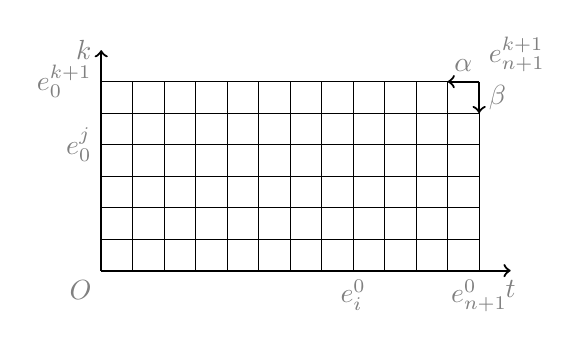
\begin{tikzpicture}[scale=0.4]
    \draw[thick,->] (0, 0) -- (13, 0); \draw[thick,->] (0, 0) -- (0,7); \draw[gray] (0,0) node[anchor=north east] {$O$};
    \draw[gray] (0,7) node[anchor=east] {$k$}; \draw[gray] (13,0) node[anchor=north] {$t$}; \draw[gray] (0,4)
    node[anchor=east] {$e_{0}^{j}$}; \draw[gray] (0,6) node[anchor=east] {$e_{0}^{k+1}$}; \draw[gray] (8,0)
    node[anchor=north] {$e_{i}^{0}$}; \draw[gray] (12,0) node[anchor=north] {$e_{n+1}^{0}$}; \draw[gray] (12,6)
    node[anchor=south west] {$e_{n+1}^{k+1}$}; \foreach \y in {1,2,3,4,5,6} \draw (0,\y) -- (12,\y); \foreach \x in
    {1,2,3,4,5,6,7,8,9,10,11,12} \draw (\x,0) -- (\x,6); \draw[thick,->] (12,6) -- (12, 5); \draw[thick,->] (12,6) --
    (11, 6); \draw[gray] (11.5,6) node[anchor=south] {$\alpha$}; \draw[gray] (12,5.5) node[anchor=west] {$\beta$};
  \end{tikzpicture}
  \caption{误差关系 $e_{n+1}^{k+1}=\alpha e_{n}^{k+1} + \beta e_{n+1}^{k}$}
  \label{fig:error}
\end{figure}

这里选取一点作为例子来说明.想要将 $e_{n+1}^{k+1}$ 移动到 $e_{i}^{0}$, 需要向西移动 $n+1-i$ 步,向南移动 $k+1$ 步.每向西移动一步需要乘以因子 $\alpha$, 每向南移动一步需要乘以因子 $\beta$. 所有可能的路径数为 $\binom{k+n+2-i}{k+1}$, 所以有 $\beta^{k+1} \binom{k+n+2-i}{k+1} \alpha^{n+1-i}e_{i}^{0}$. 类似地,为了移动到 $e_{0}^{j}$, 有 $\alpha^{n+1} \binom{n+k+2-j}{n+1} \beta^{k+1-j}e_{0}^{j}$. 把这些结果加起来,就证明了该结论.

从引理 \ref{lem:error} 可以看出,能够得到一个波形松弛方法误差的精确公式.对于波形松弛方法来说,所有的 $e_{0}^{j}$ 都为零.所以能够得到隐式欧拉波形松弛方法上面的误差结果.

证毕.

\begin{theorem}
\emph{隐式欧拉波形松弛方法的误差为
\begin{equation*}
    e_{n+1}^{k+1}=\beta^{k+1} \sum_{i=1}^{n+1} \binom{k+n+2-i}{k+1} \alpha^{n+1-i}e_{i}^{0},
  \end{equation*}
  式中 $e_{n}^{k}=y_{n}^{k}-y_{n}$, $\displaystyle{\alpha = \frac{1}{1+\Delta t m}}$, 和
  $\displaystyle{\beta = \frac{\Delta t n}{1+\Delta t m}}$.}
\end{theorem}

{\textbf{证明}} 因为所有的 $e_{0}^{j}$ 都为零,该结果可以由引理 \ref{lem:error} 自然得到.

证毕.

\begin{theorem}
  \emph{隐式欧拉波形松弛方法的误差可以用如下式子来控制
  \begin{equation*}
    \| e_{n+1}^{k+1} \| \le \frac{\beta^{k+1} e}{(1-\alpha)^{k+2}},
  \end{equation*}
  式中 $e=\max\limits_{1\le i \le n+1} \|e_{i}^{0}\|$.}
\end{theorem}

{\textbf{证明}} 由下面的几何级数公式
  \begin{equation*}
    \frac{1}{(1-\alpha)^{k+1}}=\sum_{n=0}^{\infty}\binom{k+n}{n}\alpha^n,
  \end{equation*}
  能够得到,如果取 $e=\max\limits_{1\le i \le n+1} \|e_{i}^{0}\|$, 就有
  \begin{equation*}
    \| e_{n+1}^{k+1} \| \le \frac{\beta^{k+1} e}{(1-\alpha)^{k+2}}.
  \end{equation*}

证毕.

从这个定理可以看到,随着 $\beta/(1-\alpha)$ 的减小,误差也在减小.注意到
$\alpha = 1/(1+\Delta t m)$ 和 $\beta = (\Delta t n)/(1+\Delta t m)$, 有
$\beta/(1-\alpha)=n/m$. 事实也是如此,因为当 $n=0$ 时,就是所收敛到的离散格式.

%\subsection{窗口加速技术}
%\esubsection{Windowing Accelerating Technique}
窗口加速技术是由 \cite{zhang1996note} 提出,并在 \cite{jiang2006windowing} 中详细分析的.窗口的长度需要根据所能容忍的误差来决定.取定窗口长度之后,就可以挨个窗口逐次求解了.窗口技术具有天然的可并行性,如图 \ref{fig:para1} 所示.

\begin{figure}[h]
  \centering
  \begin{tikzpicture}[scale=0.5]
    \draw[thick,->] (0, 0) -- (16, 0); \draw[thick,->] (0, 0) -- (0,6); \draw[thick] (0,0) node[anchor=north east] {$O$};
    \draw[thick] (0,6) node[anchor=east] {$k$}; \draw[thick] (16,0) node[anchor=north] {$t$}; \foreach \y in {1,2,3,4}
    \draw (0,\y) -- (15.5,\y); \foreach \x in {1,2,3,4,5,6,7,8,9,10,11,12,13,14,15} \draw (\x,0) -- (\x,4); \draw[thick]
    (5,0) -- (5, 4.5); \draw[thick] (10,0) -- (10, 4.5); \draw[thick] (15,0) -- (15, 4.5); \draw[thick] (2.5,4)
    node[anchor=south] {Window 1}; \draw[thick] (7.5,4) node[anchor=south] {Window 2}; \draw[thick] (12.5,4)
    node[anchor=south] {Window 3}; \draw[thick] (0,4) node[anchor=east] {$k$th iter}; \foreach \z in {0,5,10}{
      \draw[thick,->,-triangle 90] (\z+0,1) -- (\z+1,0); \draw[thick,->,-triangle 90] (\z+0,2) -- (\z+2,0);
      \draw[thick,->,-triangle 90] (\z+0,3) -- (\z+3,0); \draw[thick,->,-triangle 90] (\z+0,4) -- (\z+4,0);
      \draw[thick,->,-triangle 90] (\z+1,4) -- (\z+5,0); \draw[thick,->,-triangle 90] (\z+2,4) -- (\z+5,1);
      \draw[thick,->,-triangle 90] (\z+3,4) -- (\z+5,2); \draw[thick,->,-triangle 90] (\z+4,4) -- (\z+5,3); }
  \end{tikzpicture}
  \caption{窗口技术及其并行策略}
  \label{fig:para1}
\end{figure}

在图 \ref{fig:para1} 中可以看到,窗口之间的技术是串行的,但是,在每个``箭头''上,是可以并行求解的.如果记迭代次数为 $k$, 记每个窗口的时间节点数为 $N$, 那么,需要 $k+N-1$ 步并行的计算.如果串行求解,需要 $Nk$ 步的计算时间.因此,理论的加速比为 $(Nk)/(k+N-1)$.

此外,窗口大小可以由以下公式得到 \cite{jiang2006windowing}
\begin{equation*}
  T_\epsilon=\max\Bigg\{t:\sqrt[k_s]{\int_a^te^{(t-s)L_1}\frac{(t-s)^{k_s-1}}{(k_s-1)!}\,\mathrm{d}s}\le \varepsilon/L_2,\quad t>a\Bigg\},
\end{equation*}
式中 $L_1$ 和 $L_2$ 是由分裂函数所产生的常数, $k_s$ 是每个窗口最大的迭代次数, $a$ 是每个窗口的初始时刻, $\varepsilon$ 是所能容许的误差.

由 \cite{jiang2006windowing} 可知,窗口大小可以取为等间距的,这对于辛方法来说是有利的一个方面,因为取等时间步长是保证长时间计算结果稳定的一个必要条件 \cite{hairer2006geometric}. 这一点是由半群理论所得到的.

\section{流形上基于波形松弛的李群方法}\label{sec:04wrmani}
\esection{Lie Group Method Based on the WR Method on Manifolds}

在这一节里,将介绍适用于一些特定流形上计算的数值方法.该类方法利用了在流形上的作用的李群结构,和其相切的线性空间,即李代数,以及指数映射.

首先考虑这样一类矩阵方程
\begin{equation*}
	y'=A(t)y,\quad t\geq 0,\quad y(0)=y_0,
\end{equation*}
式中 $y_0\in \mathbb{R}^n,\forall t \geq 0,$ $A(t)$ 是一个 $n\times n$ 矩阵.

对于 $n=1$ 的情况,该方程的解可以直接积分得到
\begin{equation*}
	y(t)=e^{\int_0^ta(\xi)d\xi}y_0.
\end{equation*}

然而,对于 $n>1$ 的情况,上面形式的解就不再是方程的解了,只有在满足可交换条件时才能成立.

对于数值解法,正如前面所陈述,对于一个流形上的解,数值结果会远离该流形,导致数值结果不满足理论结果,这并不是我们想要的.因此,有必要重新考虑利用李群的理论,将数值结果限制在该流形上.

在本节,要考虑的是这样一类李群方程
\begin{equation*}
	Y'=A(t,Y)Y,\quad t\geq 0,\quad Y(0)=Y_0,
\end{equation*}
式中 $Y_0\in G $, $A:\mathbb{R}^+\times G\to \mathfrak{g}$, 它的解满足
\begin{equation*}
	Y(t)\in G,\quad t\geq 0.
\end{equation*}

对于这类方程,有几个经典的例子.
\begin{description}
	\item[(1) 正交矩阵流] 满足如下条件的微分方程被称作正交流
	\begin{equation*}
		Y'=A(t,Y)Y,\quad t\geq 0,\quad Y(0)=Y_0\in O(N),
	\end{equation*}
	式中 $A:\mathbb{R}^+\times O(N)\to \mathfrak{so}(N)$. 可以知道对于任意的 $t\geq 0$, 该方程的解 $Y(t)$ 是一个正交矩阵.
	\item[(2) 等谱矩阵流] 满足如下条件的微分方程被称作等谱流
	\begin{equation*}
		Y'=B(t,Y)Y-YB(t,Y),\quad t\geq 0,\quad Y(0)=Y_0\in S_N,
	\end{equation*}
	式中 $B:\mathbb{R}^+\times S_N\to \mathfrak{so}(N)$. 可以知道,该方程的解析解 $Y(t)$ 的特征值随时间保持不变.
\end{description}

\subsection{流形上的李群方法}
\esubsection{Lie Group Method on Manifolds}
这一节,从矩阵李群的概念入手,逐步得到求解流形上微分方程的 Crouch-Grossman 方法和 RK-MK 方法.

\subsubsection{矩阵李群基本概念}
\esubsubsection{Introduction to Matrix Lie Groups}

首先,要对矩阵李群进行讨论.
\begin{definition}
	\emph{一个实数的矩阵李群,是一个光滑的子集 $\mathcal{G}\subseteq \mathbb{R}^{n\times n}$, 在矩阵乘积和矩阵求逆下封闭.记 $I\in \mathcal{G}$ 为单位矩阵.}
\end{definition}

李群的李代数是李群在单位元上的切空间,因此有
\begin{definition}
	\emph{李群 $\mathcal{G}$ 的李代数 $\mathfrak{g}$ 是一个线性子空间 $\mathfrak{g}\subseteq \mathbb{R}^{n\times n}$ 包含了如下形式的所有矩阵
	\begin{equation*}
		\mathfrak{g} = \left\lbrace A \in \mathbb{R}^{n\times n}:A=\left.\frac{d\rho(s)}{ds}\right|_{s=0}\right\rbrace,
	\end{equation*}
	式中 $\rho(s)\in \mathcal{G}$ 是一个光滑曲线,满足 $\rho(0)=I$. 该空间 $\mathfrak{g}$ 在矩阵乘积,标量相乘和矩阵交换子
	\begin{equation*}
		[A,B]=AB-BA,
	\end{equation*}
	下封闭.}
\end{definition}

有了矩阵李群和李代数,就可以定义在矩阵李群上的微分方程.
\begin{definition}
	\emph{在矩阵李群上的微分方程具有如下的形式
	\begin{equation*}
		Y'=A(t,Y)Y,\quad t\geq 0,\quad Y(0)\in \mathcal{G},
	\end{equation*}
	式中 $A:\mathbb{R}\times \mathcal{G}\to \mathfrak{g}$, 并且 $AY$ 就是 $A\in \mathfrak{g}$ 和 $Y\in \mathcal{G}$ 之间的矩阵乘积.}
\end{definition}

对于指数映射,它的形式和指数函数的定义类似.
\begin{definition}
	\emph{矩阵李代数到李群的指数映射 $\mbox{expm}:\mathfrak{g}\to\mathcal{G}$ 定义为
	\begin{equation*}
		\mbox{expm}(A)=\sum_{j=0}^{\infty}\frac{A^j}{j!}.
	\end{equation*}}
\end{definition}

注意到 $\mbox{expm}(O)=I$, 并且对于充分靠近 $O\in \mathfrak{g}$ 的 $A$, 都有一个光滑的逆,记作 $\mbox{logm}:\mathcal{G}\to\mathfrak{g}$.

\begin{definition}
	\emph{矩阵的伴随表示 $\mbox{Ad}$ 和它的导数 $\mbox{ad}$ 有如下定义
	\begin{equation*}
		\mbox{Ad}_P(A)=PAP^{-1},
	\end{equation*}
	\begin{equation*}
		\mbox{ad}_A(B)=AB-BA=[A,B].
	\end{equation*}}
\end{definition}

\begin{definition}
	\emph{指数映射的微分是指数映射的右平凡化切向量,即如下的函数 $\mbox{dexp}:\mathfrak{g}\times \mathfrak{g}\to \mathfrak{g}$, 满足
	\begin{equation*}
		\frac{d}{dt}\exp(A(t))=\mbox{dexp}_{A(t)}(A'(t))\exp(A(t)).
	\end{equation*}}
\end{definition}

事实上,对于固定的 $A(t)$, 可以看出来 $\mbox{Ad}_A,\mbox{ad}_A,\mbox{dexp}_A$ 都是线性映射.因此,在 $\mathfrak{g}$ 上都可以看作是矩阵.这里的 $\mbox{dexp}_A$ 是一个解析函数
\begin{equation*}
	\mbox{dexp}_A=\frac{\mbox{expm}(\mbox{ad}_A)-I}{\mbox{ad}_A}.
\end{equation*}

该函数可以用指数函数展开
\begin{equation*}
	\begin{aligned}
		\mbox{dexp}_A(C)&=C+\frac{1}{2!}[A,C]+\frac{1}{3!}[A,[A,C]]+\frac{1}{4!}[A,[A,[A,C]]]+\cdots\\
		&=\sum_{j=0}^{\infty}\frac{1}{(j+1)!}\mbox{ad}^j_AC.
	\end{aligned}
\end{equation*}

这里,更需要的是该函数的逆
\begin{equation*}
	\mbox{dexp}_A^{-1}=\frac{\mbox{ad}_A}{\mbox{expm}(\mbox{ad}_A)-I}.
\end{equation*}

对其逆的展开,需要考虑函数
\begin{equation*}
	\frac{x}{e^x-1}=1-\frac{1}{2}x+\frac{1}{12}x^2-\frac{1}{720}x^4+\cdots=\sum_{j=0}^{\infty}\frac{B_j}{j!}x^j,
\end{equation*}
式中 $B_j$ 是伯努利数.伯努利数在解析数论的黎曼猜想里有着重要的作用.因此,有如下展开
\begin{equation*}
	\mbox{dexp}_A^{-1}(C)=C-\frac{1}{2}[A,C]+\frac{1}{12}[A,[A,C]]+\cdots=\sum_{j=0}^{\infty}\frac{B_j}{j!}\mbox{ad}^j_AC.
\end{equation*}

接下来说明该函数展开的作用,首先给出如下定义
\begin{definition}
	\emph{给定一个函数 $\psi:\mathfrak{g}\to\mathcal{G}$, 其右平凡化切向量被定义为 $d\psi:\mathfrak{g} \times \mathfrak{g} \to \mathfrak{g}$ 满足
	\begin{equation*}
		\frac{d}{dt}\psi(A(t))=d\psi_{A(t)}(A'(t))\psi(A(t)).
	\end{equation*}}
\end{definition}

然后通过 $\mbox{dexp}^{-1}$ 来求得 Baker–Campbell–Hausdorff(BCH) 公式.定义一个函数 $bch:\mathfrak{g} \times \mathfrak{g} \to \mathfrak{g}$ 满足
\begin{equation*}
	\mbox{expm}(bch(A,B))=\mbox{expm}(A)\mbox{expm}(B).
\end{equation*}

为了计算 $C=bch(A,B)$, 把它写成微分方程.令 $C(t)=bch(tA,B)$. 显然有 $C(0)=B$, 用此来计算 $C(t)$. 把式
\begin{equation*}
	\mbox{expm}(C(t))=\mbox{expm}(tA)\mbox{expm}(B)
\end{equation*}
对 $t$ 求微分,有
\begin{equation*}
	\mbox{dexp}_{C(t)}(C'(t))\exp(C(t))=\mbox{dexp}_{tA}\exp(tA)\exp(B)=A~\exp(C(t)),
\end{equation*}
因此有
\begin{equation*}
	C'(t)=\mbox{dexp}_{C(t)}^{-1}(A).
\end{equation*}

于是,得到如下定理
\begin{theorem}[BCH 公式 \cite{arieh2005liegroup}]
	\emph{函数 $C=bch(A,B)$ 可以由如下的微分方程来计算
	\begin{equation*}
		C'(t)=\mbox{dexp}_{C(t)}^{-1}(A),\quad 0\leq t\leq 1,\quad C(0)=B,
	\end{equation*}
	式中 $C(1)=bch(A,B)$.}
\end{theorem}

可以看到,该微分方程右端的式子,可以由前面的展开式得到近似,这对于设计求解李群方程的数值方法有着重要的作用,也就引出了我们的李群方法.

关于流形上的李群方法,通常来说有两种手段,一种是 Crouch-Grossman 方法 \cite{crouch1993numerical,klein2013numerical,munthe2013onpost,sonneville2014geome,bras2011anonlinear,kroshko2011integrating} ,另一种是 RK-MK \cite{arieh2005liegroup} 方法.

\subsubsection{Crouch-Grossman 方法}
\esubsubsection{The Crouch-Grossman Methods}
Crouch-Grossman(CG) 方法可以说是李群数值方法的带头人,该方法是较早提出的流形上的优秀的数值方法.有趣的是,该方法最初的应用是机器人和控制理论.

从本质上讲,该算法是将 Runge-Kutta 方法作用到李群方程上的一个有效尝试.该方法通过不断地冻结和融化系数,保证了解的流在流形的配置空间上.

该方法的基本思想是,先沿着一个方向走一小步,然后利用指数映射,将结果投射到流形上.每次都这样,直到完成一整步 Runge-Kutta 的步骤.因此,经过一个 CG 方法迭代,数值结果还在流形上.尽管该结果也会带来误差,但是不会脱离流形.

对比 Runge-Kutta 法, Crouch-Grossman 方法的基本形式是
\begin{equation*}
\left.\begin{aligned}
		X_k&=e^{ha_{k,k-1}F_{k-1}}e^{ha_{k,k-2}F_{k-2}}\cdots e^{ha_{k,1}F_{1}}Y_n\\
		F_k&=A(t_n+c_kh,X_k)\\
		Y_{n+1}&=e^{hb_{\nu}F_{\nu}}e^{hb_{\nu-1}F_{\nu-1}}\cdots e^{hb_{1}F_{1}}Y_n
	\end{aligned}\right\rbrace\quad k=1,2,\ldots,\nu.
\end{equation*}

可以看出来,该方法是一个显式方法.一个早先的三步三阶方法 \cite{crouch1993numerical} 是
\begin{equation*}
	\begin{aligned}
		X_1&=Y_n,\\
		F_1&=A(t_n,X_1),\\
		X_2&=e^{\frac{3}{4}hF_1}Y_n,\\
		F_2&=A(t_n+\frac{3}{4}h,X_2),\\
		X_3&=e^{\frac{17}{108}hF_2}e^{\frac{119}{216}hF_1}Y_n,\\
		F_2&=A(t_n+\frac{17}{24}h,X_3),\\
		Y_{n+1}&=e^{\frac{13}{51}hF_3}e^{-\frac{2}{3}hF_2}e^{\frac{24}{17}hF_1}Y_n.
	\end{aligned}
\end{equation*}

后来,有人将其推广到隐式方法,隐式方法需要将上面的 $X_k$ 变成
\begin{equation*}
	X_k=e^{ha_{k,\nu}F_{\nu}}e^{ha_{k,\nu-1}F_{\nu-1}}\cdots e^{ha_{k,1}F_{1}}Y_n,\quad k=1,2,\ldots,\nu.
\end{equation*}

隐式方法的缺点是求解流形上的隐式问题更加复杂.

\subsubsection{RK-MK 方法}
\esubsubsection{The Runge-Kutta-Munthe-Kaas Methods}
相比之下, RK-MK 方法(又叫做 RK-MK 类方法)更加实用.这类方法及其理论由陆续的几篇文章 \cite{mk1996lie,mk1997numerical,mk1998runge,mk1999high} 建立起来.该方法和 CG 方法类似,利用了指数映射.不同的是, CG 方法每走一小步都要求落回到流形上, RK-MK 方法先在李代数这个线性空间上进行计算,最后用指数映射保证这一步的计算结果在流形上.

该方法建立在如下的理论上.
\begin{theorem}[指数映射的微分 \cite{arieh2005liegroup}]
	\emph{对于很小的 $t\geq 0$, 李群方法的解有如下的形式
	\begin{equation*}
		Y(t)=\mbox{expm}(\Theta(t))Y_0,
	\end{equation*}
	式中 $\Theta \in \mathfrak{g}$ 满足微分方程
	\begin{equation*}
		\Theta'(t)=\mbox{dexp}_{\Theta(t)}^{-1}(A(t,Y))\quad \Theta(0)=O,
	\end{equation*}
	这里的 $\mbox{dexp}$ 为指数映射的微分.}
\end{theorem}

该定理告诉我们,如果能够求得 $\Theta(t)$, 代入这个解,就可以求得李群方程的解.首先,给出 Butcher 表
\begin{center}
  \begin{tabular}{c|cccc}
    $c_1$&$a_{11}$&$a_{12}$&$\cdots$&$a_{1\nu}$\\
    $c_2$&$a_{21}$&$a_{22}$&$\cdots$&$a_{2\nu}$\\
    $\vdots$&$\vdots$&$\vdots$&$\ddots$&$\vdots$\\
    $c_{\nu}$&$a_{\nu 1}$&$a_{\nu 2}$&$\cdots$&$a_{\nu \nu}$\\
    \hline
         &$b_{1}$&$b_{2}$&$\cdots$&$b_{\nu}$
  \end{tabular}
\end{center}
式中 $a,b,c$ 为 Runge-Kutta 法里的常数. RK-MK 法利用了 RK 法的基本思想,结合了李群指数映射的特性,具有比较好的数值效果.
\begin{equation*}
	\begin{aligned}
		&\left.\begin{aligned}
		\Theta_k&=\sum_{l=1}^{\nu}a_{k,l}F_l,\\
		A_k&=hA(t_n+c_kh,\mbox{expm}(\Theta_k)Y_n),\\
		F_k&=\mbox{dexp}_{\Theta_k}^{-1}(A_k),
	\end{aligned}\right\rbrace \quad k=1,2,\ldots,\nu\\
		&\begin{aligned}
		\Theta&=\sum_{l=1}^{\nu}b_lF_l,\\
		Y_{n+1}&=\mbox{expm}(\Theta)Y_n.
	\end{aligned}
	\end{aligned}
\end{equation*}

实际应用中,这里的 $\mbox{dexp}_{\Theta_k}^{-1}(A_k)$ 可以用前面的展开式进行计算,为了简化,这里只需展开几项进行计算.

需要注意的是,为了计算 $\mbox{ad}^j_AC$, 需要如下递推公式得到
\begin{equation*}
	\mbox{ad}^0(u)(v)=v,
\end{equation*}
\begin{equation*}
	\mbox{ad}^n(u)(v)=\mbox{ad}(u)(\mbox{ad}^{n-1}(u)(v))=[u,[u,[\cdots,[u,v]]]],\quad \forall n \geq 1.
\end{equation*}

展开的项数可以根据如下定理选取.
\begin{theorem}[RK-MK 方法阶数 \cite{qin2011struc}]
	\emph{若 Runge-Kutta 方法有 $p$ 阶, $\mbox{dexp}^{-1}$ 展开式中取到 $q$ 项,且 $q\geq p-1$, 则相应的 RK-MK 方法为 $p$ 阶的.}
\end{theorem}

这里给出一个 RK-MK 方法的例子.对于如下的 Butcher 表
\begin{center}
  \begin{tabular}{c|cccc}
    $0$&&&&\\
    $\frac{1}{2}$&$\frac{1}{2}$&&&\\
    $\frac{1}{2}$&$0$&$\frac{1}{2}$&&\\
    $1$&$0$&$0$&$1$&\\
    \hline
         &$\frac{1}{6}$&$\frac{1}{3}$&$\frac{1}{3}$&$\frac{1}{6}$
  \end{tabular}
\end{center}

则对应的 $4$ 阶精度的 RK-MK 法如下
\begin{equation*}
	\begin{aligned}
		&\psi_1=0,\\
		&A_1=hA(t_n,y_n),\\
		&K_1=A_1,\\
		&\psi_2=\frac{1}{2}K_1,\\
		&A_2=hA(t_n+\frac{1}{2}h,e^{\psi_2}y_n),\\
		&K_2=A_2-\frac{1}{2}[\psi_2,A_2]+\frac{1}{12}[\psi_2,[\psi_2,A_2]],\\
		&\psi_3=\frac{1}{2}K_2,\\
		&A_3=hA(t_n+\frac{1}{2}h,e^{\psi_3}y_n),\\
		&K_3=A_3-\frac{1}{2}[\psi_3,A_3]+\frac{1}{12}[\psi_3,[\psi_3,A_3]],\\
		&\psi_4=K_3,\\
		&A_4=hA(t_n+h,e^{\psi_4}y_n),\\
		&K_4=A_4-\frac{1}{2}[\psi_4,A_4]+\frac{1}{12}[\psi_4,[\psi_4,A_4]],\\
		&y_{n+1}=\exp(\frac{1}{6}K_1+\frac{1}{3}K_2+\frac{1}{3}K_3+\frac{1}{6}K_4)y_n.
	\end{aligned}
\end{equation*}

可以看出,和 CG 方法相比,这种方法减少了指数映射的计算次数,因此就减少了计算量和精度分析的难度.

注意到,上面的方法是显式的,这样的计算是很容易的.但如果一个李群方程不仅要求数值结果在流形上,而且要求该数值方法保持某些结构,可能需要一些隐式方法来求解.这个问题类比于哈密尔顿系统,有一个守恒量,用上面显式的方法只能保证结果在流形上,却无法保证在流形上有保结构的结果.

对于上面的不足,如果要求保证守恒性质,需要隐式的 RK-MK 方法,我们利用波形松弛方法对其进行显式改造.

%\section{流形上的波形松弛方法}\label{sec:04wrmani}
%\esection{Waveform Relaxation Methods on Manifolds}

\subsection{主要方法讨论}
\esubsection{Discussions on the Main Method}

在本小节,给出隐式的 RK-MK 方法的一个波形松弛改造,首先回归到 RK-MK 的基本算法上
\begin{equation*}
	\begin{aligned}
		&\left.\begin{aligned}
		\Theta_k&=\sum_{l=1}^{\nu}a_{k,l}F_l,\\
		A_k&=hA(t_n+c_kh,\mbox{expm}(\Theta_k)Y_n),\\
		F_k&=\mbox{dexp}_{\Theta_k}^{-1}(A_k),
	\end{aligned}\right\rbrace \quad k=1,2,\ldots,\nu\\
		&\begin{aligned}
		\Theta&=\sum_{l=1}^{\nu}b_lF_l,\\
		Y_{n+1}&=\mbox{expm}(\Theta)Y_n.
	\end{aligned}
	\end{aligned}
\end{equation*}

这里面最重要的是最后一步的更新
\begin{equation*}
	Y_{n+1}=\mbox{expm}(\Theta)Y_n,
\end{equation*}
此处的 $\Theta$ 为李代数上的更新,指数映射将其拉回流形上.前三项循环的部分主要是为了求解 $F_k$, 可以通过代入得到关于 $F_k$ 的代数方程
\begin{equation*}
	F_k=\mbox{dexp}_{\Theta_k}^{-1}(hA(t_n+c_kh,\mbox{expm}(\sum_{l=1}^{\nu}a_{k,l}F_l)Y_n)).
\end{equation*}

因此,该算法可以写成
\begin{equation*}
	\begin{aligned}
		\Theta_k&=\sum_{l=1}^{\nu}a_{k,l}F_l,\quad k=1,2,\ldots,\nu,\\
		F_k&=\mbox{dexp}_{\Theta_k}^{-1}(hA(t_n+c_kh,\mbox{expm}(\sum_{l=1}^{\nu}a_{k,l}F_l)Y_n)),\quad k=1,2,\ldots,\nu,\\
		Y_{n+1}&=\mbox{expm}(\sum_{l=1}^{\nu}b_lF_l)Y_n.
	\end{aligned}
\end{equation*}

可以看到,隐式的 RK-MK 方法就是先求解 $F_k,k=1,2,\ldots,\nu$ 然后代入最后一个式子.

参考辛 Runge-Kutta 波形松弛方法的形式 \cite{bellen1993use} 来设计这里的算法,主要问题是如何使得格式容易计算
\begin{equation*}
  \left\lbrace
    \begin{aligned}
      Y_{n+1}^{r,(k+1)}&=\eta^{(k+1)}(t_{n})+h\sum_{s=1}^{\nu}a_{rs}F(t_{n+1}^{s},Y_{n+1}^{s,(k+1)},Y_{n+1}^{s,(k)}),\quad r=1,\cdots, \nu, \\
      \eta^{(k+1)}(t_{n+1})&=\eta^{(k+1)}(t_{n})+h\sum_{s=1}^{\nu}b_{s}F(t_{n+1}^{s},Y_{n+1}^{s,(k+1)},Y_{n+1}^{s,(k)}).
    \end{aligned}
  \right.
\end{equation*}

要对其中一步
\begin{equation*}
	F_k=\mbox{dexp}_{\Theta_k}^{-1}(hA(t_n+c_kh,\mbox{expm}(\sum_{l=1}^{\nu}a_{k,l}F_l)Y_n)),\quad k=1,2,\ldots,\nu,
\end{equation*}
进行改造,把它展开即
\begin{equation*}
	\begin{aligned}
		F_1&=\mbox{dexp}_{\Theta_1}^{-1}(hA(t_n+c_1h,\mbox{expm}(\sum_{l=1}^{\nu}a_{1,l}F_l)Y_n)),\\
		F_2&=\mbox{dexp}_{\Theta_2}^{-1}(hA(t_n+c_2h,\mbox{expm}(\sum_{l=1}^{\nu}a_{2,l}F_l)Y_n)),\\
		&\cdots \\
		F_{\nu}&=\mbox{dexp}_{\Theta_{\nu}}^{-1}(hA(t_n+c_{\nu}h,\mbox{expm}(\sum_{l=1}^{\nu}a_{\nu,l}F_l)Y_n)),
	\end{aligned}
\end{equation*}
式中 $\Theta_k=\sum_{l=1}^{\nu}a_{k,l}F_l,\quad k=1,2,\ldots,\nu$.

这里,一方面要考虑上面方程里 $F_k$ 的求解,另一方面要考虑最后的步进公式的设置
\begin{equation*}
	Y_{n+1}=\mbox{expm}(\sum_{l=1}^{\nu}b_lF_l)Y_n.
\end{equation*}

如果采用 Picard 波形松弛格式,该算法可以写成
\begin{equation*}
	\left\lbrace\begin{aligned}
		F_1^{n+1,(k+1)}&=\mbox{dexp}_{\Theta_1^{n+1,(k)}}^{-1}(hA(t_n+c_1h,\mbox{expm}(\sum_{l=1}^{\nu}a_{1,l}F_l^{n+1,(k)})Y_n^{(k)})),\\
		F_2^{n+1,(k+1)}&=\mbox{dexp}_{\Theta_2^{n+1,(k)}}^{-1}(hA(t_n+c_2h,\mbox{expm}(\sum_{l=1}^{\nu}a_{2,l}F_l^{n+1,(k)})Y_n^{(k)})),\\
		\cdots \\
		F_{\nu}^{n+1,(k+1)}&=\mbox{dexp}_{\Theta_{\nu}^{n+1,(k)}}^{-1}(hA(t_n+c_{\nu}h,\mbox{expm}(\sum_{l=1}^{\nu}a_{\nu,l}F_l^{n+1,(k)})Y_n^{(k)})),\\
		Y_{n+1}^{(k+1)}&=\mbox{expm}(\sum_{l=1}^{\nu}b_lF_l^{n+1,(k)})Y_n^{(k)},
	\end{aligned}\right.
\end{equation*}
式中 $\Theta_m^{n+1,(k)} = \sum_{l=1}^{\nu}a_{m,l}F_l^{n+1,(k)}$, $F_l^{n+1,(k)}$ 中的下指标 $l$ 是 Runge-Kutta 的步数, 上指标 $k$ 为波形松弛方法的步数, 上指标 $n+1$ 是时间节点序数.

如果采用 Gauss-Jacobi 波形松弛格式,该算法可以写成
\begin{equation*}
	\left\lbrace\begin{aligned}
		F_1^{n+1,(k+1)}&=\mbox{dexp}_{\Theta_1^{n+1,(k)}}^{-1}(hA(t_n+c_1h,\mbox{expm}(a_{1,1}F_1^{n+1,(k+1)}+\sum_{l=1,l\neq 1}^{\nu}a_{1,l}F_l^{n+1,(k)})Y_n^{(k)})),\\
		F_2^{n+1,(k+1)}&=\mbox{dexp}_{\Theta_2^{n+1,(k)}}^{-1}(hA(t_n+c_2h,\mbox{expm}(a_{2,2}F_2^{n+1,(k+1)}+\sum_{l=1,l\neq 2}^{\nu}a_{2,l}F_l^{n+1,(k)})Y_n^{(k)})),\\
		\cdots \\
		F_{\nu}^{n+1,(k+1)}&=\mbox{dexp}_{\Theta_{\nu}^{n+1,(k)}}^{-1}(hA(t_n+c_{\nu}h,\mbox{expm}(a_{\nu,\nu}F_{\nu}^{n+1,(k+1)}+\sum_{l=1,l\neq \nu}^{\nu}a_{\nu,l}F_l^{n+1,(k)})Y_n^{(k)})),\\
		Y_{n+1}^{(k+1)}&=\mbox{expm}(\sum_{l=1}^{\nu}b_lF_l^{n+1,(k)})Y_n^{(k)},
	\end{aligned}\right.
\end{equation*}
式中 $\Theta_m^{n+1,(k)} = F_{m}^{n+1,(k+1)}+\sum_{l=1,l\neq m}^{\nu}a_{m,l}F_l^{n+1,(k)}$.

如果采用 Gauss-Seidel 波形松弛格式,该算法可以写成
\begin{equation*}
	\left\lbrace\begin{aligned}
		F_1^{n+1,(k+1)}&=\mbox{dexp}_{\Theta_1^{n+1,(k)}}^{-1}(hA(t_n+c_1h,\mbox{expm}(a_{1,1}F_1^{n+1,(k+1)}+\sum_{l=2}^{\nu}a_{1,l}F_l^{n+1,(k)})Y_n^{(k)})),\\
		F_2^{n+1,(k+1)}&=\mbox{dexp}_{\Theta_2^{n+1,(k)}}^{-1}(hA(t_n+c_2h,\mbox{expm}(\sum_{l=1}^{2}a_{2,l}F_l^{n+1,(k+1)}+\sum_{l=3}^{\nu}a_{2,l}F_l^{n+1,(k)})Y_n^{(k)})),\\
		\cdots \\
		F_{\nu}^{n+1,(k+1)}&=\mbox{dexp}_{\Theta_{\nu}^{n+1,(k)}}^{-1}(hA(t_n+c_{\nu}h,\mbox{expm}(\sum_{l=1}^{\nu}a_{\nu,l}F_{l}^{n+1,(k+1)})Y_n^{(k)})),\\
		Y_{n+1}^{(k+1)}&=\mbox{expm}(\sum_{l=1}^{\nu}b_lF_l^{n+1,(k)})Y_n^{(k)},
	\end{aligned}\right.
\end{equation*}
式中 $\Theta_m^{n+1,(k)} = \sum_{l=1}^{m}a_{m,l}F_{l}^{n+1,(k+1)}+\sum_{l=m+1}^{\nu}a_{m,l}F_l^{n+1,(k)}$.

也可以设计比 Gauss-Seidel 格式更简单的格式
\begin{equation*}
	\left\lbrace\begin{aligned}
		F_1^{n+1,(k+1)}&=\mbox{dexp}_{\Theta_1^{n+1,(k)}}^{-1}(hA(t_n+c_1h,\mbox{expm}(\sum_{l=1}^{\nu}a_{1,l}F_l^{n+1,(k)})Y_n^{(k)})),\\
		F_2^{n+1,(k+1)}&=\mbox{dexp}_{\Theta_2^{n+1,(k)}}^{-1}(hA(t_n+c_2h,\mbox{expm}(a_{2,1}F_1^{n+1,(k+1)}+\sum_{l=2}^{\nu}a_{2,l}F_l^{n+1,(k)})Y_n^{(k)})),\\
		\cdots \\
		F_{\nu}^{n+1,(k+1)}&=\mbox{dexp}_{\Theta_{\nu}^{n+1,(k)}}^{-1}(hA(t_n+c_{\nu}h,\mbox{expm}(\sum_{l=1}^{\nu-1}a_{\nu,l}F_{l}^{n+1,(k+1)}+a_{\nu,\nu}F_{\nu}^{n+1,(k)})Y_n^{(k)})),\\
		Y_{n+1}^{(k+1)}&=\mbox{expm}(\sum_{l=1}^{\nu}b_lF_l^{n+1,(k)})Y_n^{(k)},
	\end{aligned}\right.
\end{equation*}
式中 $\Theta_m^{n+1,(k)} = \sum_{l=1}^{m-1}a_{m,l}F_{l}^{n+1,(k+1)}+\sum_{l=m}^{\nu}a_{m,l}F_l^{n+1,(k)}$.

%\subsection{基本算法}
%\esubsection{Algorithm}
为了得到较好的计算格式,和辛波形松弛方法一样,还需引入窗口技术,得到如下含有多重循环的算法 \ref{alg:04sym}.

\begin{algorithm}
\caption{李群方程加窗口的波形松弛方法}
\label{alg:04sym}
\begin{algorithmic}
\STATE 初始化解矩阵
\FOR{$w= 1~\texttt{to} ~n_w$}
    \FOR{$k= 1~\texttt{to} ~n_k$}
        \FOR{$s= 1~\texttt{to} ~n_s$}
             \STATE 计算 $Y_{n+1}^{(k+1)}$.
        \ENDFOR
    \ENDFOR
\ENDFOR
\STATE 保存结果.
\end{algorithmic}
\end{algorithm}
在算法 \ref{alg:04sym} 中, $n_w$, $n_k$ 和 $n_s$ 分别代表``窗口数'',``波形松弛迭代次数''和``每个窗口的区间数''.这里需要注意保存至少两步的中间变量 $F_l^{n+1,(k)}$, 才能保证计算正确.

\section{数值实验}\label{sec:03numerical}
\esection{Numerical Experiments}
在本节,将给出四个数值算例来验证我们的算法分析.首先我们把算法的基本框架列出来,见算法 \ref{alg:sym}.

\begin{algorithm}
\caption{窗口辛波形松弛方法}
\label{alg:sym}
\begin{algorithmic}
\STATE 初始化解矩阵
\FOR{$w= 1~\texttt{to} ~n_w$}
    \FOR{$k= 1~\texttt{to} ~n_k$}
        \FOR{$s= 1~\texttt{to} ~n_s$}
             \STATE 用 \eqref{eq:discrete} 计算 $z_{n+1}^{k+1}$.
        \ENDFOR
    \ENDFOR
\ENDFOR
\STATE 保存结果.
\end{algorithmic}
\end{algorithm}

在算法 \ref{alg:sym} 中, $n_w$, $n_k$ 和 $n_s$ 分别代表``窗口数'',``波形松弛迭代次数''和``每个窗口的区间数''. 公式 \eqref{eq:discrete} 可以根据算法的不同进行替换.为了加速算法,可以进行并行计算.该算法在 $t-k$ 平面上的一个图示为图 \ref{fig:para2}.

\begin{figure}[h]
  \centering
  \begin{tikzpicture}[scale=0.5]
    \draw[thick,->] (0, 0) -- (16, 0); \draw[thick,->] (0, 0) -- (0,6); \draw[thick] (0,0) node[anchor=north east] {$O$};
    \draw[thick] (0,6) node[anchor=east] {$k$}; \draw[thick] (16,0) node[anchor=north] {$t$}; \foreach \y in {1,2,3,4}
    \draw (0,\y) -- (15.5,\y); \foreach \x in {1,2,3,4,5,6,7,8,9,10,11,12,13,14,15} \draw (\x,0) -- (\x,4); \draw[thick]
    (5,0) -- (5, 4.5); \draw[thick] (10,0) -- (10, 4.5); \draw[thick] (15,0) -- (15, 4.5); \draw[thick] (2.5,4)
    node[anchor=south] {Window 1}; \draw[thick] (7.5,4) node[anchor=south] {Window 2}; \draw[thick] (12.5,4)
    node[anchor=south] {Window 3}; \draw[thick] (0,4) node[anchor=east] {$k$th iter};
    	\foreach \y in {0,5,10}{
		\foreach \z in {0,1,2,3}{
			\draw[dashed,thick,->,-triangle 90] (\y+0,\z+0.5) -- (\y+5,\z+0.5);
		}
	}
  \end{tikzpicture}
  \caption{算法 \ref{alg:sym} 的图示}
  \label{fig:para2}
\end{figure}

\subsection*{算例 1}
考虑如下的一维 sin-Gordon 方程
\begin{equation}\label{eq:singordon}
  \left \{ \begin{array}{l}
      \displaystyle \frac{d^2 u }{d t^2} + u = -\sin u, \quad 0<t \leq t_{\text{end}},\\
      u(x, 0) = 0, \; u_t (x, 0) = 1.
    \end{array} \right.
\end{equation}
令 $q = u$ 和 $\dot{q} = p$, 可以化成如下的哈密尔顿系统
\begin{equation}\label{eq:singordonH}
  \left \{ \begin{array}{l}
      \displaystyle \frac{d q }{d t} = p,\\
      \displaystyle \frac{d p }{d t} = -q - \sin q,
    \end{array} \right.
\end{equation}
初值条件为 $q(0)=0$, $p(0)=1$, 哈密尔顿函数为
\begin{equation*}
  H(q,p) = \frac{p^2}{2} + \frac{q^2}{2} - \cos q.
\end{equation*}

首先考虑辛欧拉波形松弛方法~\eqref{eq:schemejacobi}. 取 $t_{\text{end}} = 200$, 步长为 $h = 1/100$, 波形松弛迭代次数为 $k=15$. 对于窗口加速方法,取每个时间窗口为 $1$. 图 \ref{fig:ex1seucom} 展示了辛欧拉波形松弛方法无窗口加速(a)和有窗口加速(b)的比较.发现经典的波形松弛方法需要更多的步数才能收敛.

\begin{figure}[h!]
  \centering
  \subfloat[无窗口加速]{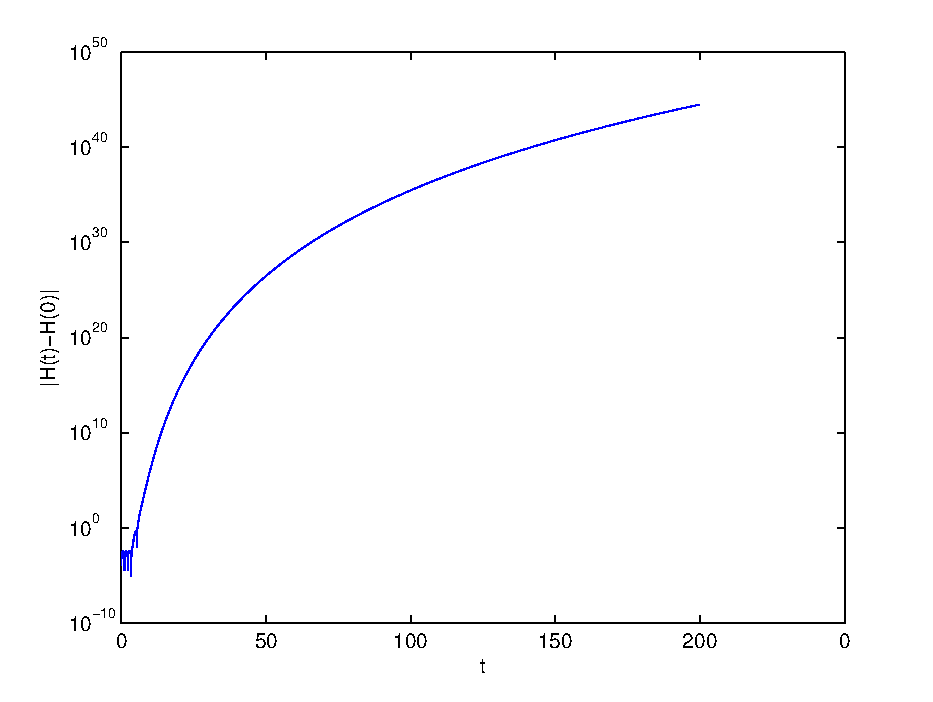
\includegraphics[width=0.45\textwidth]{03/Fig3-1.pdf}}
  \subfloat[有窗口加速]{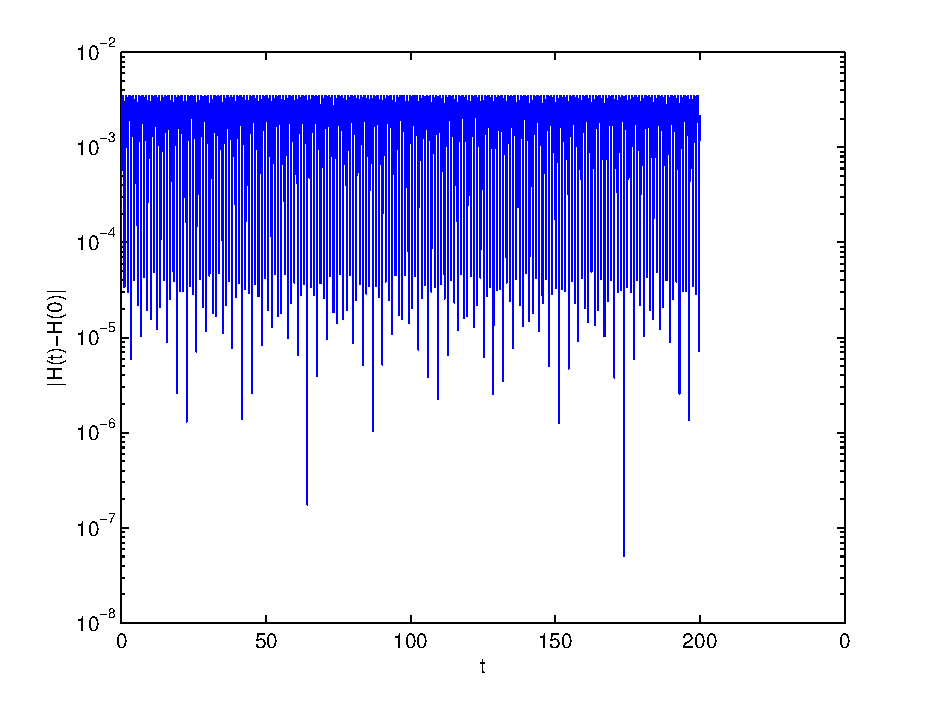
\includegraphics[width=0.45\textwidth]{03/Fig3-2.pdf}}
  \caption{sin-Gordon 方程 \eqref{eq:singordon} 辛欧拉波形松弛方法无窗口加速(a)和有窗口加速(b)的比较}
  \label{fig:ex1seucom}
\end{figure}

其次,考虑辛 Runge-Kutta 波形松弛方法~\eqref{eq:schemerkjacobi}. 取 $t_{\text{end}} = 200$, 步长为 $h = 1/100$, 波形松弛迭代次数为 $k=15$. 对于窗口加速方法,取每个时间窗口为 $1$. 图 \ref{fig:ex1srkcom} 展示了辛 Runge-Kutta 波形松弛方法无窗口加速(a)和有窗口加速(b)的比较.发现经典的波形松弛方法需要更多的步数才能收敛.在本例中使用了表 \ref{tbl:rk} 中的 Butcher 表,其中 $a = 1.351207$.

\begin{table}[h!]
  \centering
  \caption{三阶 Butcher 表}
  \label{tbl:rk}
  \begin{tabular}{c|ccc}
    $\frac{1}{2}a$ & $\frac{1}{2}a$ & & \\
    $\frac{3}{2}a$ & $a$ &$\frac{1}{2}a$  & \\
    $\frac{1}{2} + a$ & $a$ & $a$ &$\frac{1}{2}-a$\\
    \hline
    & $a$ &$a$ & $1-2a$\\
  \end{tabular}
\end{table}

\begin{figure}[h!]
  \centering
  \subfloat[无窗口加速]{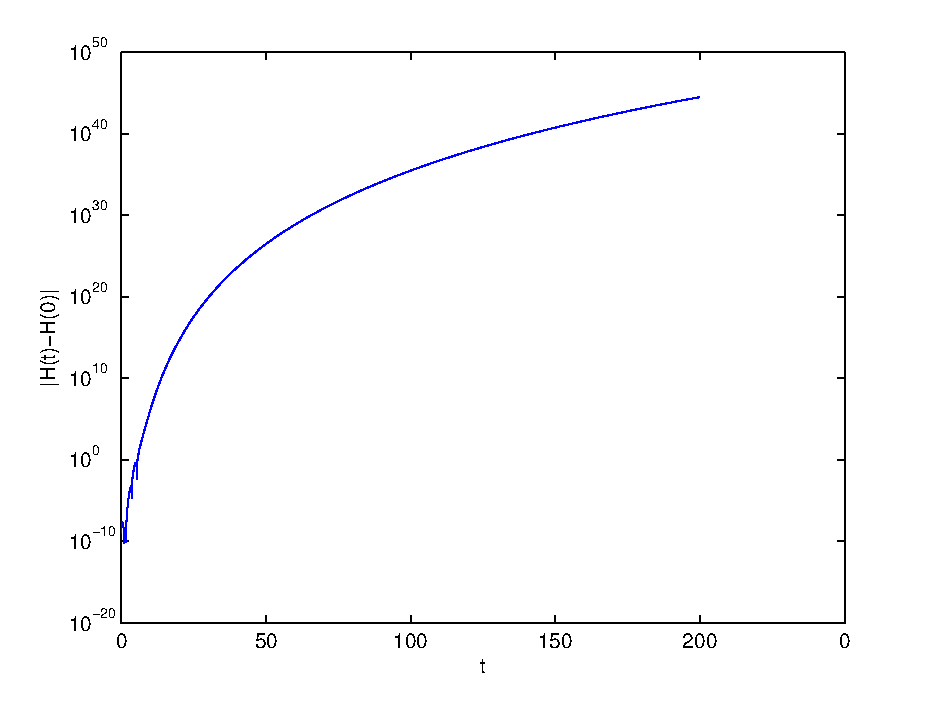
\includegraphics[width=0.45\textwidth]{03/Fig4-1.pdf}}
  \subfloat[有窗口加速]{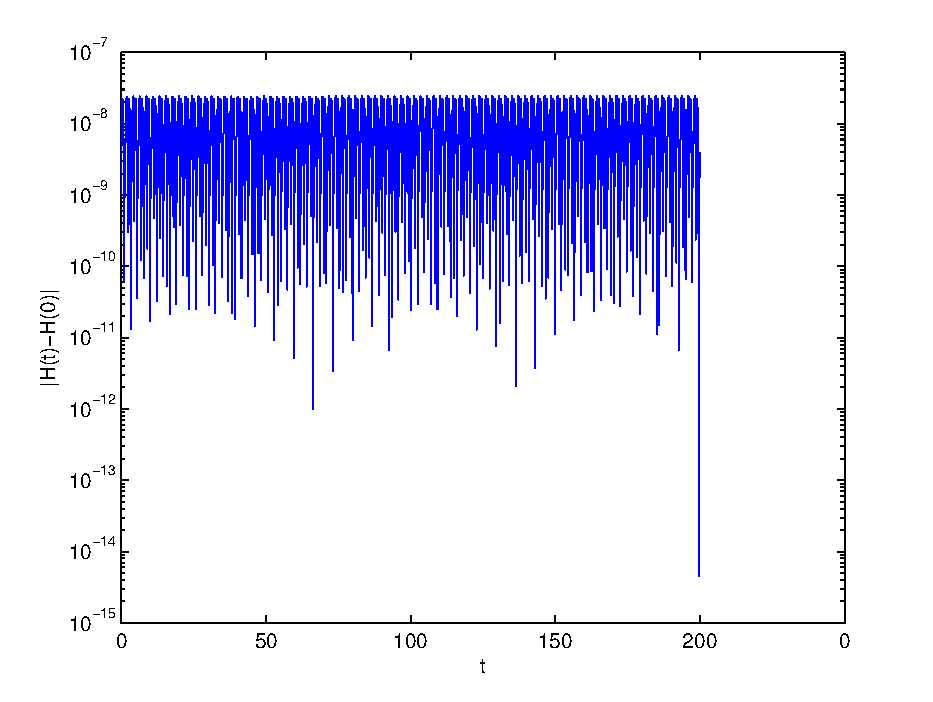
\includegraphics[width=0.45\textwidth]{03/Fig4-2.pdf}}
  \caption{sin-Gordon 方程 \eqref{eq:singordon} 辛 Runge-Kutta 波形松弛方法无窗口加速(a)和有窗口加速(b)的比较}
  \label{fig:ex1srkcom}
\end{figure}

接下来考虑辛欧拉波形松弛方法和辛 Runge-Kutta 波形松弛方法.取 $t_{\text{end}} = 200$, 步长为 $h = 1/100$, 波形松弛迭代次数为 $k=15$. 对于窗口加速方法,取每个时间窗口为 $1$. 数值结果见表 \ref{tbl:order}. 在此表中辛欧拉波形松弛方法被记作 ``seulerwrwin'',辛 Runge-Kutta 波形松弛方法被记作 ``srkwrwin''.

\begin{table}[h!]
    \begin{center}
    \caption{两种方法随时间步长 $h$ 的变化}
    \label{tbl:order}
    \begin{tabularx}{\linewidth}{XXXXX}
        \toprule[1.5pt]
        h & 4/100 & 2/100 & 1/100 & 1/200\\
        \midrule[1pt]
        seulerwrwin & 0.0143 &0.0071 &0.0035 &0.0017\\
        srkwrwin    & 1.6750e-06 & 1.9805e-07 & 2.4330e-08 & 3.3278e-09\\
        \bottomrule[1.5pt]
    \end{tabularx}
    \end{center}
  \end{table}

最后,考虑该算法的收敛性质,图 \ref{fig:ex1err} 展示了辛欧拉波形松弛方法和辛 Runge-Kutta 波形松弛方法在无窗口的情形下的收敛性质.这里,取 $t_{end} =\textbf{1}$, 步长为 $h=1/100$. 全局最大误差为 $0.0035$.

图 \ref{fig:ex1winerr} 展示了辛欧拉波形松弛方法和辛 Runge-Kutta 波形松弛方法在有窗口的情形下的收敛性质.这里,取 $t_{end} =\textbf{1}$, 步长为 $h=1/100$, 每个时间窗口为 $1$. 全局最大误差为 $2.4330e-08$.

\begin{figure}[h!]
  \centering
  \subfloat[无窗口加速]{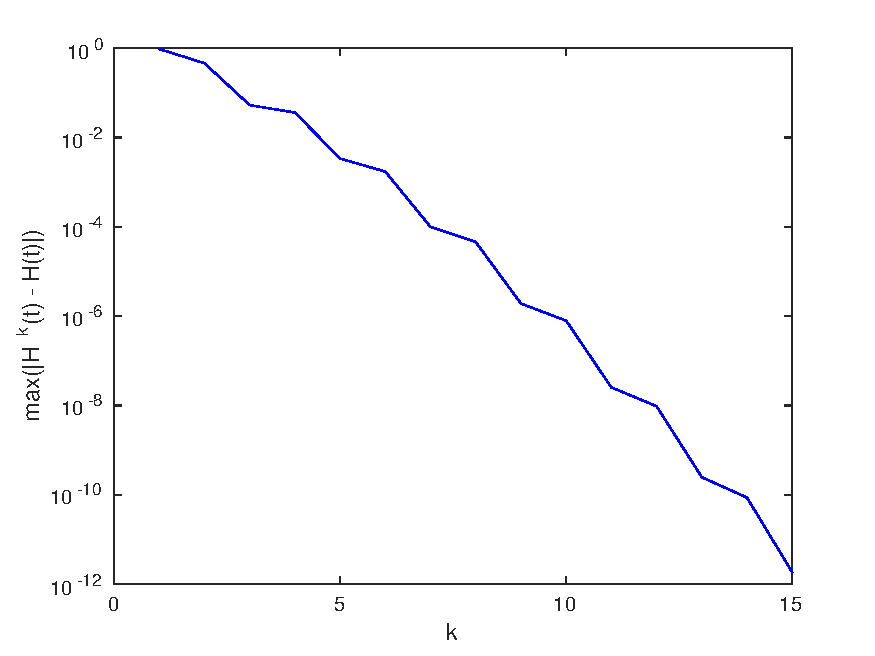
\includegraphics[width=0.45\textwidth]{03/Fig5-1.pdf}}
  \subfloat[有窗口加速]{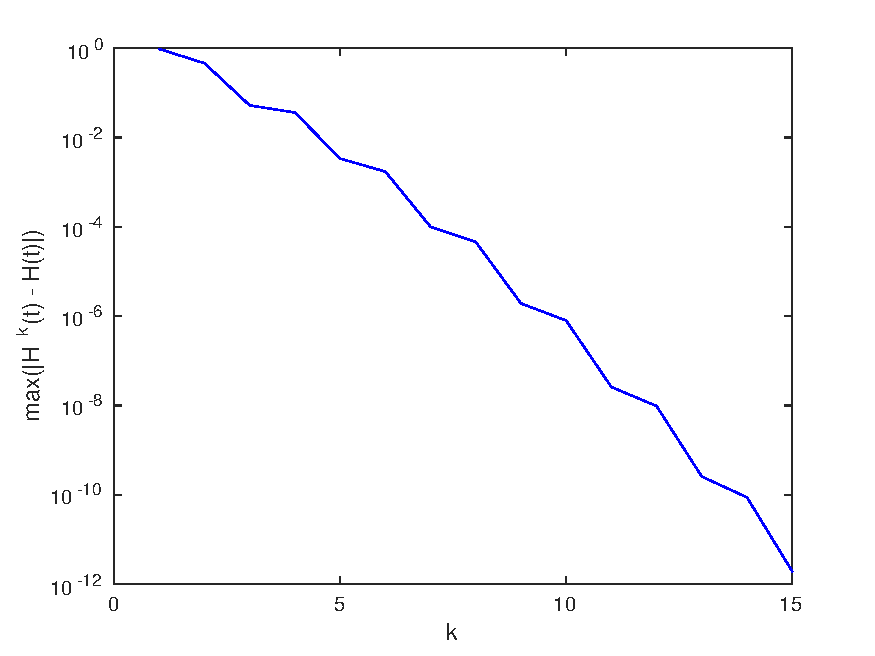
\includegraphics[width=0.45\textwidth]{03/Fig5-2.pdf}}
  \caption{sin-Gordon 方程 \eqref{eq:singordon} 辛欧拉波形松弛方法(a)和辛 Runge-Kutta 波形松弛方法(b)在无窗口的情形下的比较}
  \label{fig:ex1err}
\end{figure}

\begin{figure}[h!]
  \centering
  \subfloat[无窗口加速]{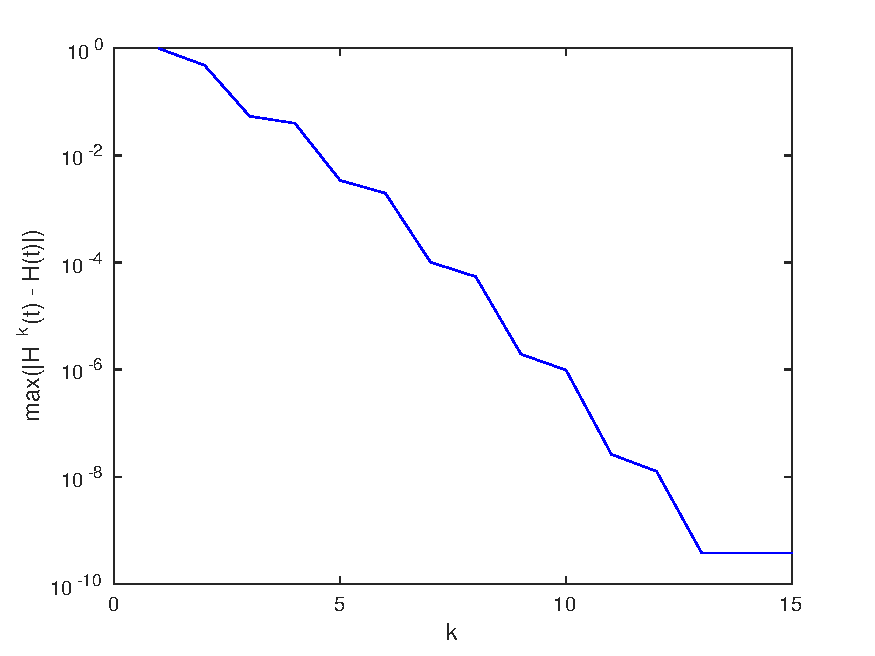
\includegraphics[width=0.45\textwidth]{03/Fig6-1.pdf}}
  \subfloat[有窗口加速]{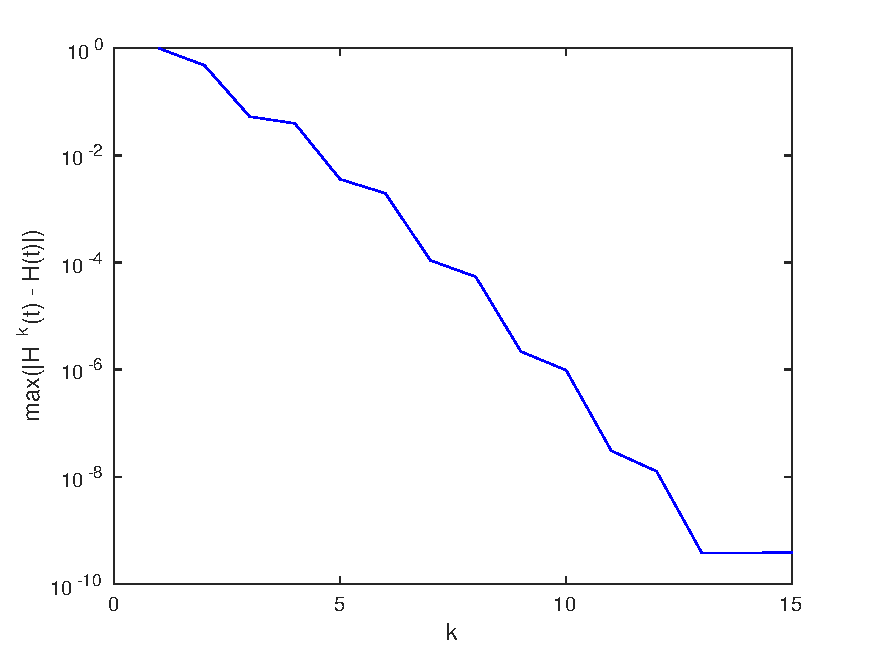
\includegraphics[width=0.45\textwidth]{03/Fig6-2.pdf}}
  \caption{sin-Gordon 方程 \eqref{eq:singordon} 辛欧拉波形松弛方法(a)和辛 Runge-Kutta 波形松弛方法(b)在有窗口的情形下的比较}
  \label{fig:ex1winerr}
\end{figure}

\subsection*{算例 2}
考虑 Fermi-Pasta-Ulam 问题 \cite{hairer2006geometric}. 其哈密尔顿函数为
\begin{equation*}
  \begin{aligned}
    H(q,p) &= \displaystyle{\frac{1}{2}} \sum_{i=1}^{2m} p_i +
    \displaystyle{\frac{\omega^2}{2}} \sum_{i=1}^{m} q_{m+i}^2 +
    \displaystyle{\frac{1}{4}}  \{ (x_1 - x_{m+1})^4 \\
    & \qquad + \sum_{i=1}^{m-1} (x_{i+1} - x_{m+i-1} - x_i - x_{m+i})^4 + (x_{m}
    - x_{2m})^4\},
  \end{aligned}
\end{equation*}
式中 $0<t\leq t_{\text{end}}$, $q_i~(i=1,2,\ldots,m)$ 为第 $i$ 个弹簧的位移,$q_{m+i}~(i=1,2,\ldots,m)$ 为第 $i$ 个弹簧拉伸或收缩的长度, $p_i~(i=1,2,\ldots,m)$ 是它们的速度,见图示~\ref{fig:fpu}.

\begin{figure}[h!]
  \centering
  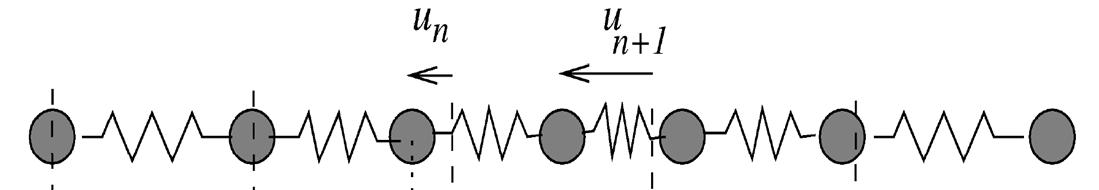
\includegraphics[width=0.6\textwidth]{03/FPUchainedependules.jpg}
  \caption{Fermi-Pasta-Ulam 示意图,图中两端固定}
  \label{fig:fpu}
\end{figure}

在本例中 \cite{hairer2006geometric}, 取 $m=3$, $\omega = 50$,
\begin{equation*}
  q_1(0) = 1, \quad p_1(0) = 1, \quad q_4(0) = \frac{1}{\omega}, \quad p_4(0) = 1,
\end{equation*}
并且其他的初值为 $0$.

首先,考虑辛欧拉波形松弛方法~\eqref{eq:schemejacobi}. 取 $t_{\text{end}} = 10$, 步长为 $h = 10^{-3}$, 波形松弛迭代次数为 $k=20$. 对于窗口加速方法,取每个时间窗口为 $0.1$. 图 \ref{fig:ex2seucom} 展示了辛欧拉波形松弛方法无窗口加速(a)和有窗口加速(b)的比较.发现经典的波形松弛方法需要更多的步数才能收敛.全局最大误差为 $0.0195$.

\begin{figure}[h!]
  \centering
  \subfloat[无窗口加速]{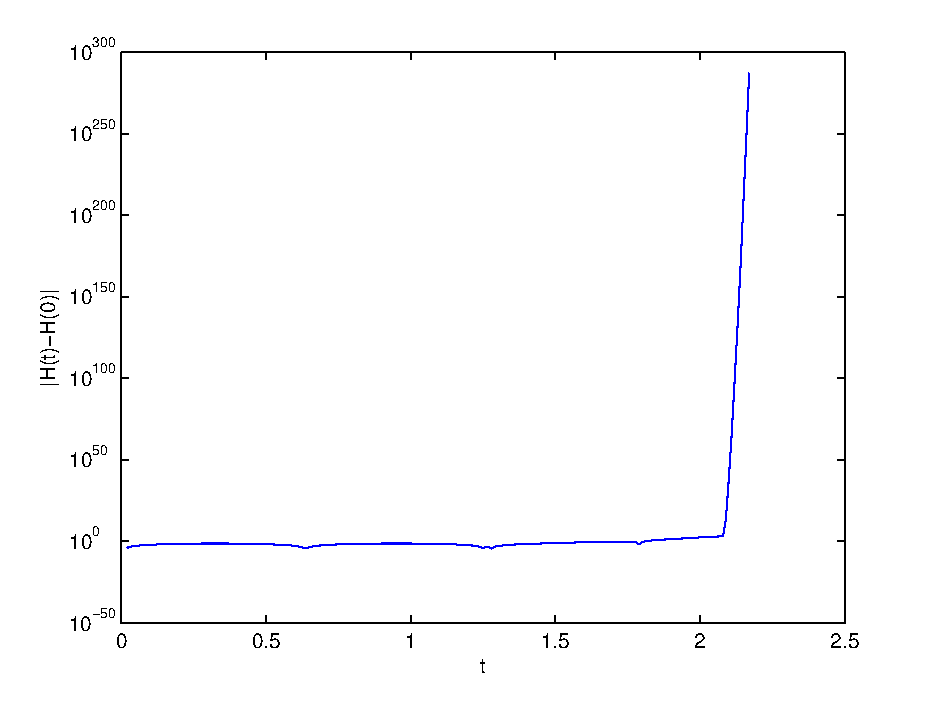
\includegraphics[width=0.45\textwidth]{03/Fig7-1.pdf}}
  \subfloat[有窗口加速]{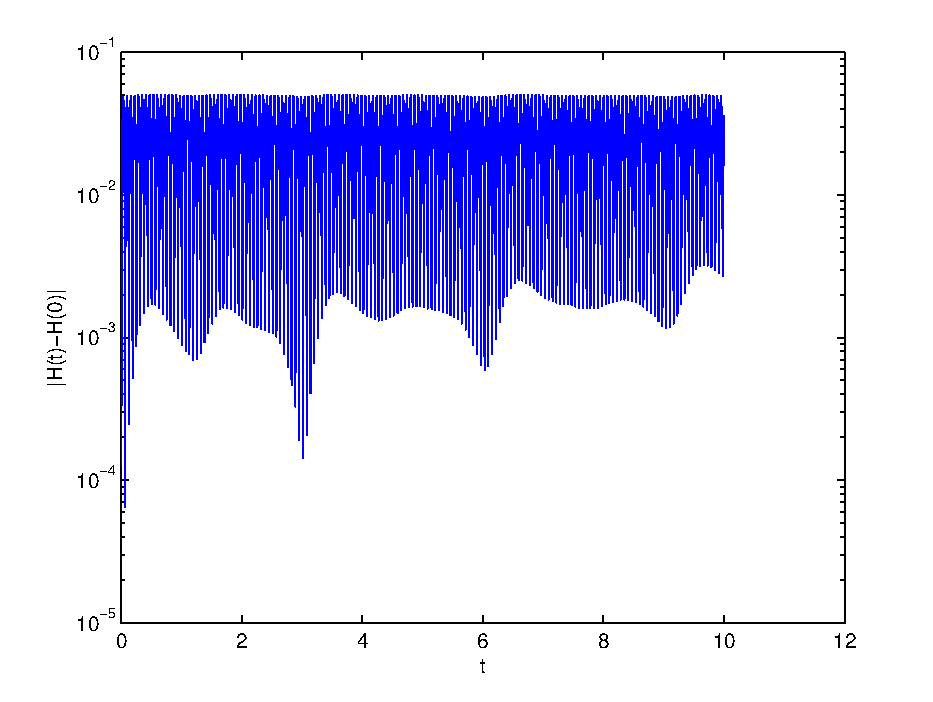
\includegraphics[width=0.45\textwidth]{03/Fig7-2.pdf}}
  \caption{Fermi-Pasta-Ulam 问题辛欧拉波形松弛方法无窗口加速(a)和有窗口加速(b)的比较}
  \label{fig:ex2seucom}
\end{figure}

之后,考虑辛 Runge-Kutta 波形松弛方法~\eqref{eq:schemerkjacobi}. 取 $t_{\text{end}} = 10$, 步长为 $h = 1/100$, 波形松弛迭代次数为 $k=30$. 对于窗口加速方法,取每个时间窗口为 $0.1$. 图 \ref{fig:ex2srkcom} 展示了辛 Runge-Kutta 波形松弛方法无窗口加速(a)和有窗口加速(b)的比较.发现经典的波形松弛方法需要更多的步数才能收敛.在本例中使用了表 \ref{tbl:rk} 中的 Butcher 表,其中 $a = 1.351207$. 全局最大误差为 $1.0948e-06$.

\begin{figure}[h!]
  \centering
  \subfloat[无窗口加速]{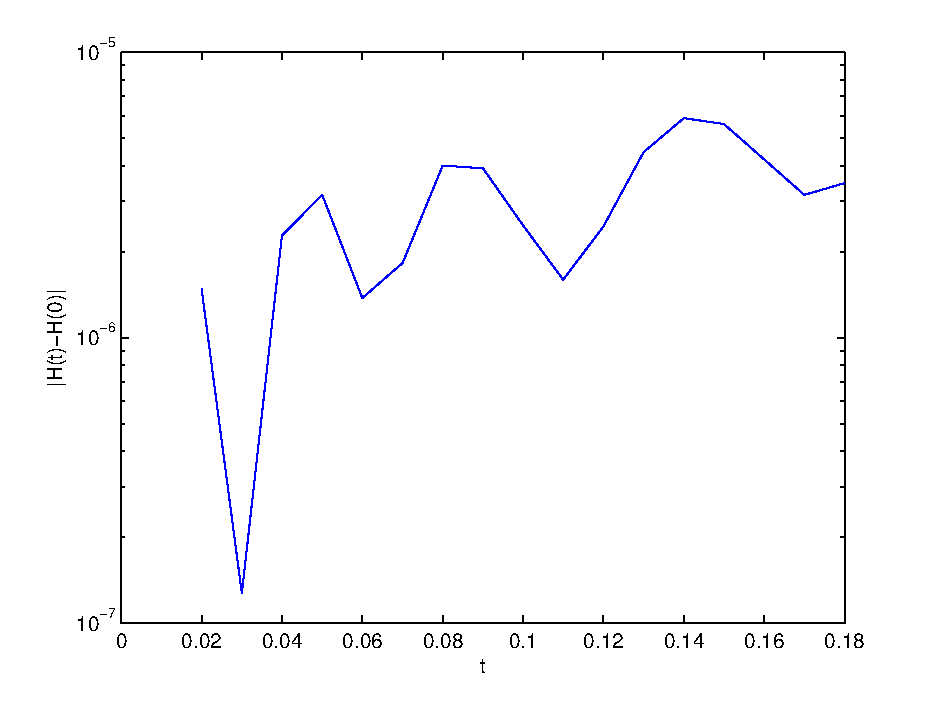
\includegraphics[width=0.45\textwidth]{03/Fig8-1.pdf}}
  \subfloat[有窗口加速]{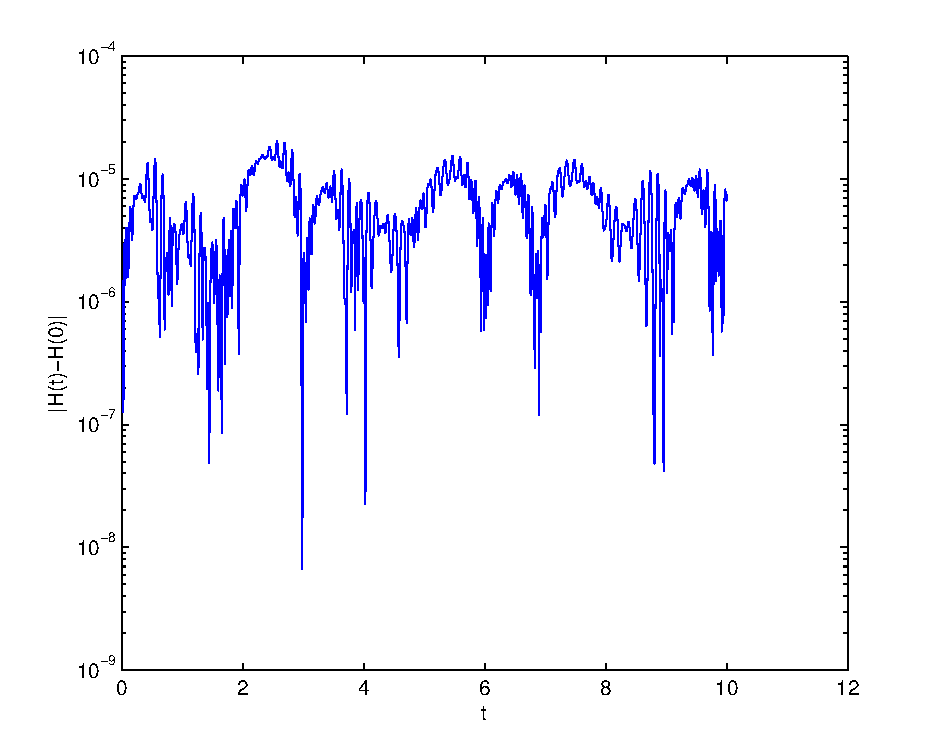
\includegraphics[width=0.45\textwidth]{03/Fig8-2.pdf}}
  \caption{Fermi-Pasta-Ulam 问题辛 Runge-Kutta 波形松弛方法无窗口加速(a)和有窗口加速(b)的比较}
  \label{fig:ex2srkcom}
\end{figure}

\subsection*{算例 3}
考虑如下的非线性波动方程 \cite{wu2013struc}
\begin{equation}\label{eq:nonlinwave}
  \left \{ \begin{array}{l}
      \displaystyle \frac{\partial^2 u }{\partial t^2}
      - \frac{\partial^2 u}{\partial x^2}
      = -\frac{1}{5} u^3 - \frac{1}{10} u^2, \quad 0<x<1, \; 0<t \leq t_{\text{end}},\\
      u(0,t) = u(1,t) = 0, \; u(x, 0) = \dfrac{\sin(\pi x)}{2}, \; u_t (x, 0) = 0.
    \end{array} \right.
\end{equation}
使用二阶中心差分方法,取空间步长为 $\Delta x = 1/N$ 和 $x_i = i \Delta x$, 得到如下的系统

\begin{equation*}
  \left \{ \begin{array}{l}
      \displaystyle \frac{d^2 U }{d t^2} + MU =F(t, U), \quad 0<t \leq t_{\text{end}},\\
      U(0) = (\dfrac{\sin(\pi x_1)}{2}, \ldots, \dfrac{\sin(\pi x_{N-1})}{2})^{T}, \quad U^{'} ={\bf 0},
    \end{array} \right.
\end{equation*}
式中 $U(t)=(u_1(t), \ldots. u_{N-1}(t))^{T}$ 和 $u_i(t) \approx u(x_i,t)$,
$x=1,2,\ldots,N-1$, 和
\begin{equation*}
  M = \frac{1}{\Delta x^2}
  \begin{pmatrix}
    2 & -1 & & &\\
    -1 & 2 & -1 & & \\
    & \ddots & \ddots& \ddots & \\
    & &-1 & 2 &-1 \\
    & & & -1&2\\
  \end{pmatrix},
\end{equation*}
\begin{equation*}
  F(t,U) = \left( -\frac{1}{5}u_1^3 -\frac{1}{10}u_1^2, \ldots,
    -\frac{1}{5}u_{N-1}^3 -\frac{1}{10}u_{N-1}^2 \right)^{T}.
\end{equation*}

令 $q := (q_1, \ldots, q_{N-1})^{T}= U$ 和 $p :=(p_1, \ldots, p_{N-1})^{T}:= \dot{q} = U^{'}$, 得到如下的哈密尔顿系统

\begin{equation}\label{eq:nonlinwaveH}
  \left \{ \begin{array}{l}
      \displaystyle \frac{d q }{d t} = p,\\
      \displaystyle \frac{d p }{d t} = -Mq - f(q),
    \end{array} \right.
\end{equation}
式中
\begin{equation*}
  f(q) = (\frac{1}{5} q_1^3 + \frac{1}{10} q_1^2, \ldots,
  \frac{1}{5} q_{N-1}^3 + \frac{1}{10} q_{N-1}^2)^{T},
\end{equation*}
初值条件为 $q(0)=(\frac{\sin(\pi x_1)}{2}, \ldots,
\frac{\sin(\pi x_{N-1})}{2})^{T}$, $p(0)={\bf 0}$, 其哈密尔顿函数为
$H(q,p) = \frac{1}{2}p^{ T}p + \frac{1}{2}q^{T}q + G(q)$, 式中
\begin{equation*}
  G(q) = \frac{1}{20} q_1^4 + \frac{1}{30} q_1^3 + \ldots + \frac{1}{20}
  q_{N-1}^4 + \frac{1}{30} q_{N-1}^3.
\end{equation*}

首先,考虑辛欧拉波形松弛方法~\eqref{eq:schemejacobi}. 取 $t_{\text{end}} = 10$, $N=20$, 步长为 $h = 10^{-3}$, 波形松弛迭代次数为 $k=10$. 对于窗口加速方法,取每个时间窗口为 $0.1$. 图 \ref{fig:ex3seucom} 展示了辛欧拉波形松弛方法无窗口加速(a)和有窗口加速(b)的比较.发现经典的波形松弛方法需要更多的步数才能收敛.全局最大误差为 $0.0506$.

\begin{figure}[h!]
  \centering
  \subfloat[无窗口加速]{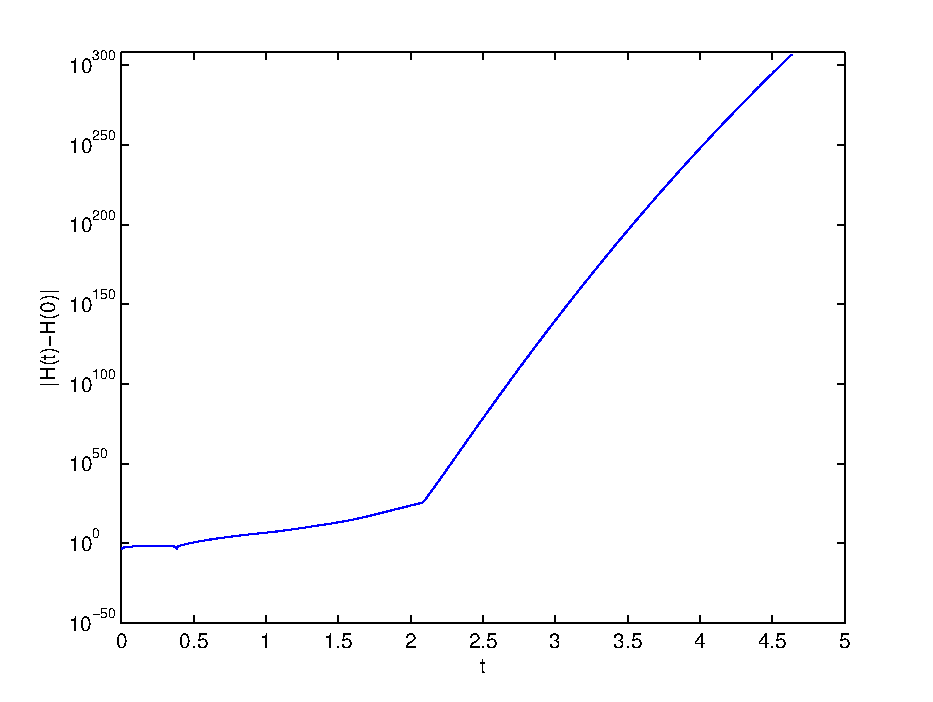
\includegraphics[width=0.45\textwidth]{03/Fig9-1.pdf}}
  \subfloat[有窗口加速]{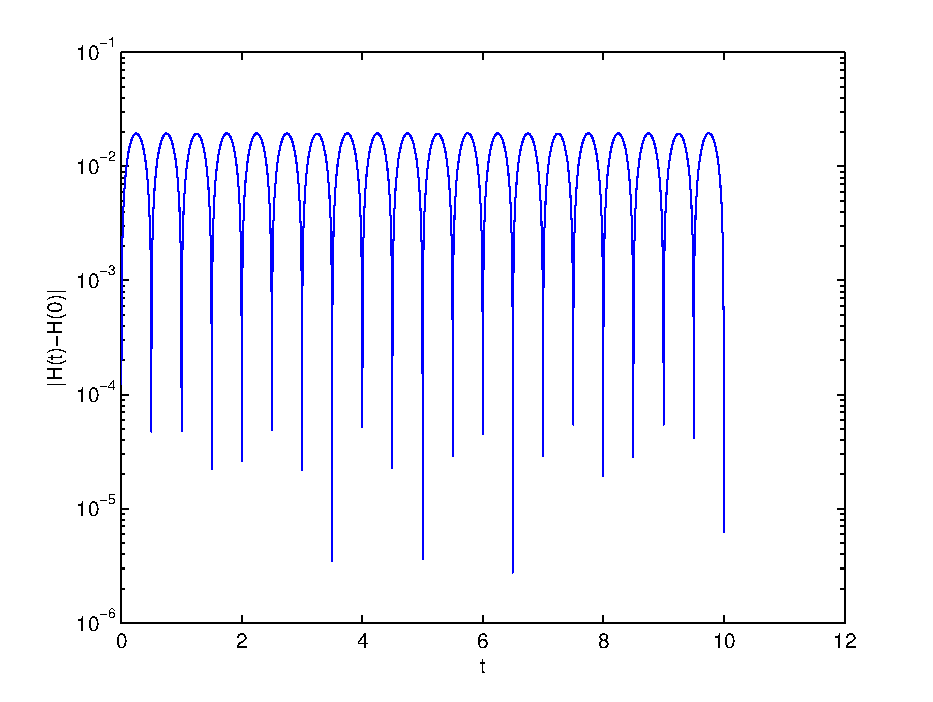
\includegraphics[width=0.45\textwidth]{03/Fig9-2.pdf}}
  \caption{非线性波动方程 \eqref{eq:nonlinwave} 辛欧拉波形松弛方法无窗口加速(a)和有窗口加速(b)的比较}
  \label{fig:ex3seucom}
\end{figure}

之后,考虑辛 Runge-Kutta 波形松弛方法~\eqref{eq:schemerkjacobi}. 取 $t_{\text{end}} = 10$, $N=20$, 步长为 $h = 1/100$, 波形松弛迭代次数为 $k=30$. 对于窗口加速方法,取每个时间窗口为 $0.1$. 图 \ref{fig:ex3srkcom} 展示了辛 Runge-Kutta 波形松弛方法无窗口加速(a)和有窗口加速(b)的比较.发现经典的波形松弛方法需要更多的步数才能收敛.在本例中使用了表 \ref{tbl:rk} 中的 Butcher 表,其中 $a = 1.351207$. 全局最大误差为 $3.7003e-05$.

\begin{figure}[h!]
  \centering
  \subfloat[无窗口加速]{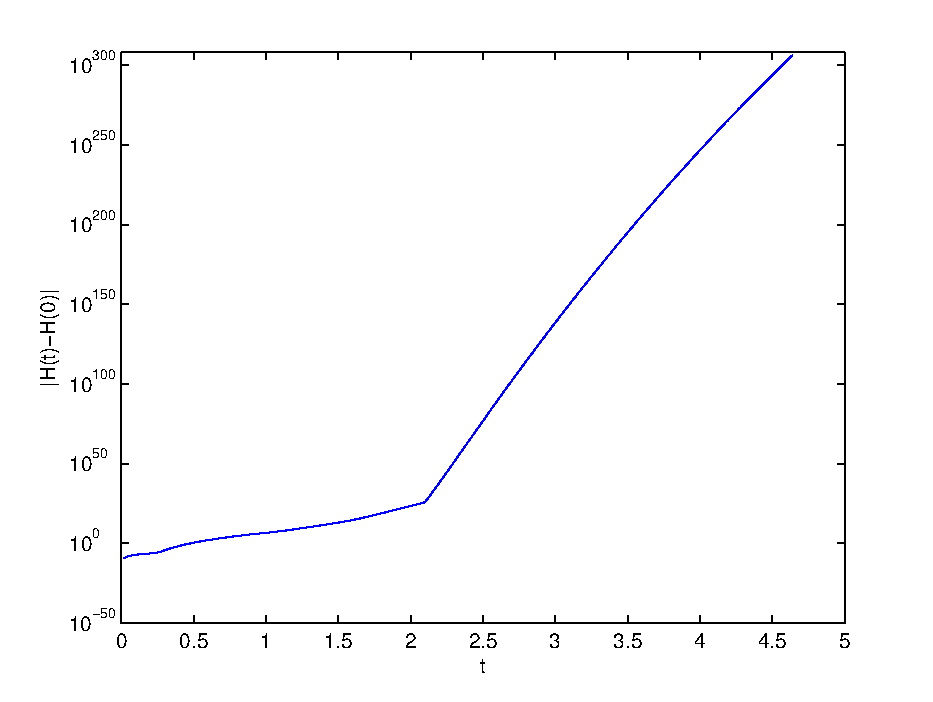
\includegraphics[width=0.45\textwidth]{03/Fig10-1.pdf}}
  \subfloat[有窗口加速]{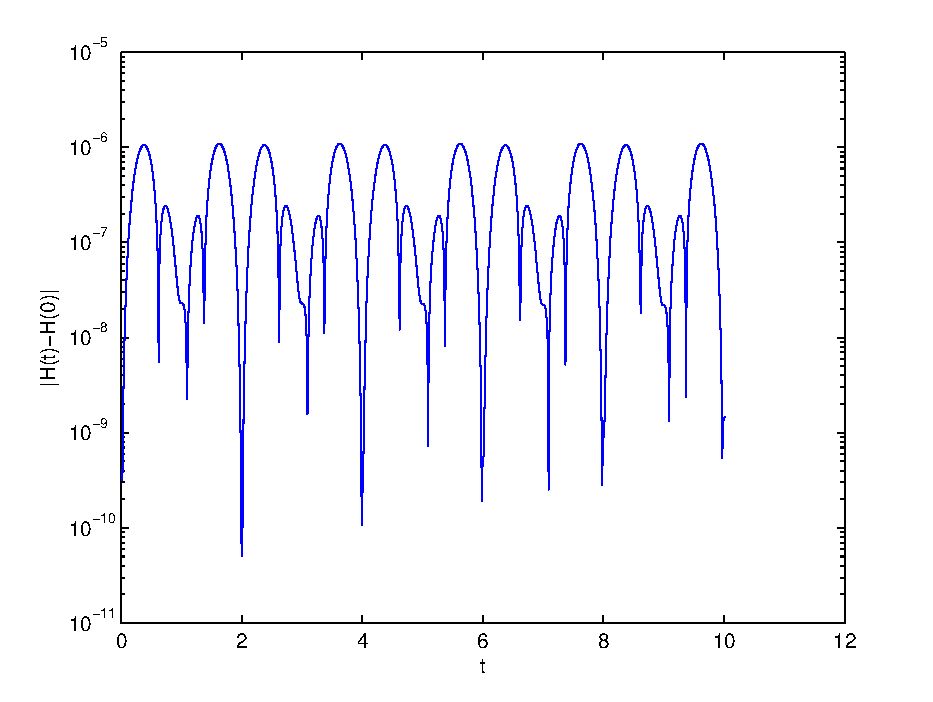
\includegraphics[width=0.45\textwidth]{03/Fig10-2.pdf}}
  \caption{非线性波动方程 \eqref{eq:nonlinwave} 辛 Runge-Kutta 波形松弛方法无窗口加速(a)和有窗口加速(b)的比较}
  \label{fig:ex3srkcom}
\end{figure}

其数值解的示意图如图 \ref{fig:wavefig}.

\begin{figure}[h!]
  \centering
  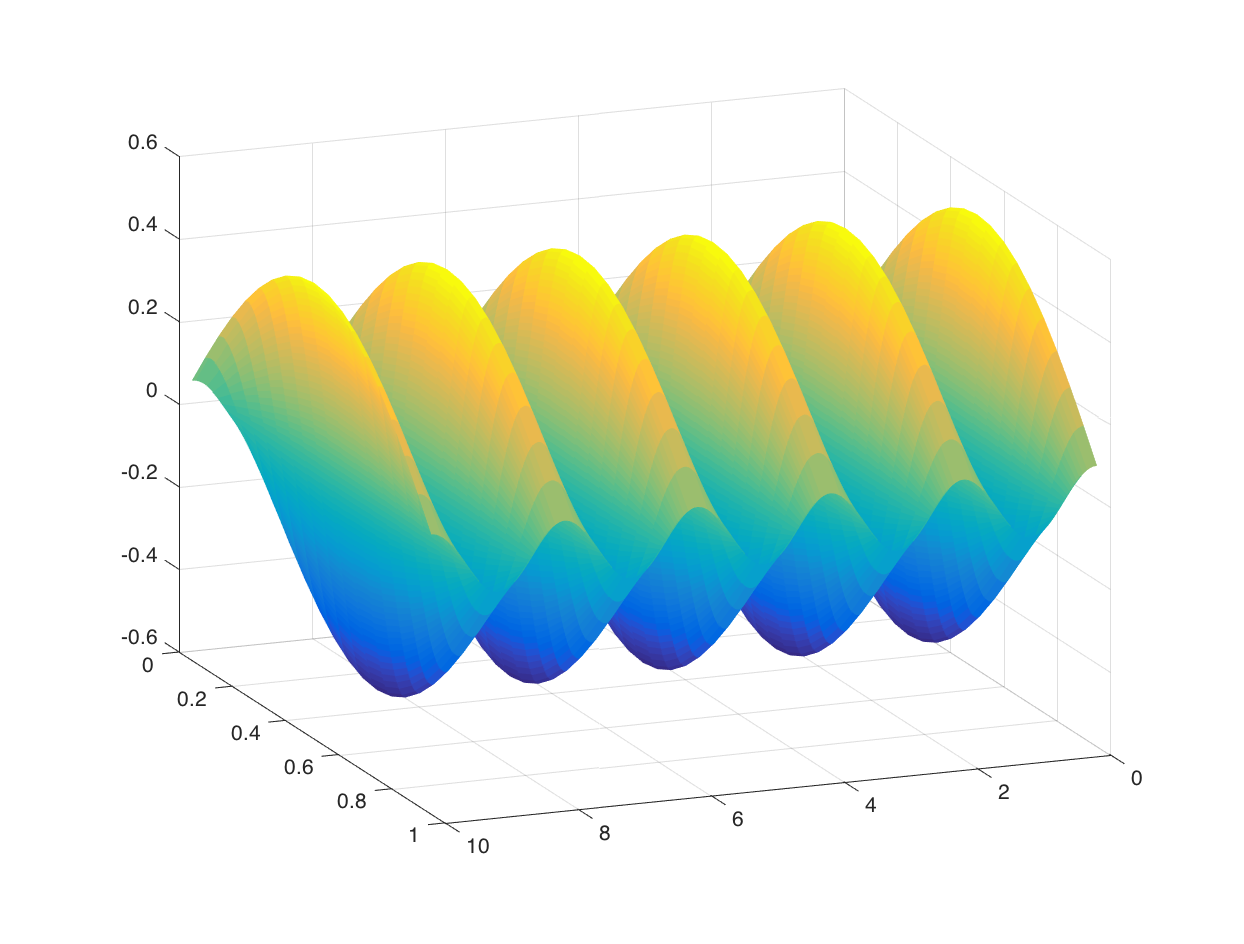
\includegraphics[width=0.6\textwidth]{03/wave.pdf}
  \caption{非线性波动方程的解示意图}
  \label{fig:wavefig}
\end{figure}

\subsection*{算例 4}
最后给出一个计算的李群方程的例子,这个例子基于如下形式的三阶常微分方程

\begin{equation*}
  	\begin{pmatrix}
  		\dot{y_1}\\ \dot{y_2}\\ \dot{y_3}
  	\end{pmatrix}=
  	\begin{pmatrix}
  		0&y_3/I_3&-y_2/I_2\\
  		-y_3/I_3&0&y_1/I_1\\
  		y_2/I_2&-y_1/I_1&0
  	\end{pmatrix}
  	\begin{pmatrix}
  	y_1\\ y_2\\ y_3
  	\end{pmatrix},
 \end{equation*}
式中 $I_1,~I_2,~I_3$ 为常数.或者等价地写成
\begin{equation*}
  	\begin{aligned}
  		\dot{y_1}&=a_1 y_2 y_3,\qquad a_1=(I_2-I_3)/(I_2I_3),\\
  		\dot{y_2}&=a_2 y_3 y_1,\qquad a_3=(I_3-I_1)/(I_3I_1),\\
  		\dot{y_3}&=a_3 y_1 y_2,\qquad a_3=(I_1-I_2)/(I_1I_2).
  	\end{aligned}
\end{equation*}
根据李群方程的形式,可以知道
\begin{equation*}
  	A(t,Y)=
  	\begin{pmatrix}
  		0&y_3/I_3&-y_2/I_2\\
  		-y_3/I_3&0&y_1/I_1\\
  		y_2/I_2&-y_1/I_1&0
  	\end{pmatrix}.
 \end{equation*}

该问题描述了刚体的自由运动,其质心在中点.该系统有两个守恒量,可以通过如下计算得到.首先根据如下的式子
\begin{equation*}
	a_1+a_2+a_3=(\frac{1}{I_3}-\frac{1}{I_2})+(\frac{1}{I_1}-\frac{1}{I_3})+(\frac{1}{I_2}-\frac{1}{I_1})=0,
\end{equation*}
得到守恒量
\begin{equation*}
	{y_1}^2+{y_2}^2+{y_3}^2.
\end{equation*}
再根据
\begin{equation*}
	\frac{a_1}{I_1}+\frac{a_2}{I_2}+\frac{a_3}{I_3}=\frac{(I_2-I_3)+(I_3-I_1)+(I_1-I_2)}{I_1I_2I_3}=0,
\end{equation*}
可以得到守恒量
\begin{equation*}
	H(y_1,y_2,y_3)=\frac{1}{2}(\frac{{y_1}^2}{I_1}+\frac{{y_2}^2}{I_2}+\frac{{y_3}^2}{I_3}).
\end{equation*}

可以看到,第一个守恒量描述刚体的形状不变,第二个则描述动能守恒.该问题的解可以看作是一个球体和一个椭球的交线,因此,该解在一个稳定的椭圆上.

算例中,使用表 \ref{tbl:04rk3} 中的 Butcher 表,该表对应的 Runge-Kutta 法是一个辛方法,其中 $a = 1.351207$.

\begin{table}[h!]
  \centering
  \caption{三阶 Butcher 表}
  \label{tbl:04rk3}
  \begin{tabular}{c|ccc}
    $\frac{1}{2}a$ & $\frac{1}{2}a$ & & \\
    $\frac{3}{2}a$ & $a$ &$\frac{1}{2}a$  & \\
    $\frac{1}{2} + a$ & $a$ & $a$ &$\frac{1}{2}-a$\\
    \hline
    & $a$ &$a$ & $1-2a$\\
  \end{tabular}
\end{table}

通过计算,能得到如下的数值结果,如图 \ref{fig:rkmk3}. 可以看出,该方法能够保持原格式应有的效果,得到了一个保结构的数值算法.这里,取步长为 $0.3$, 共取了 $500$ 步,分 $10$ 个窗口计算.

\begin{figure}[h!]
  \centering
  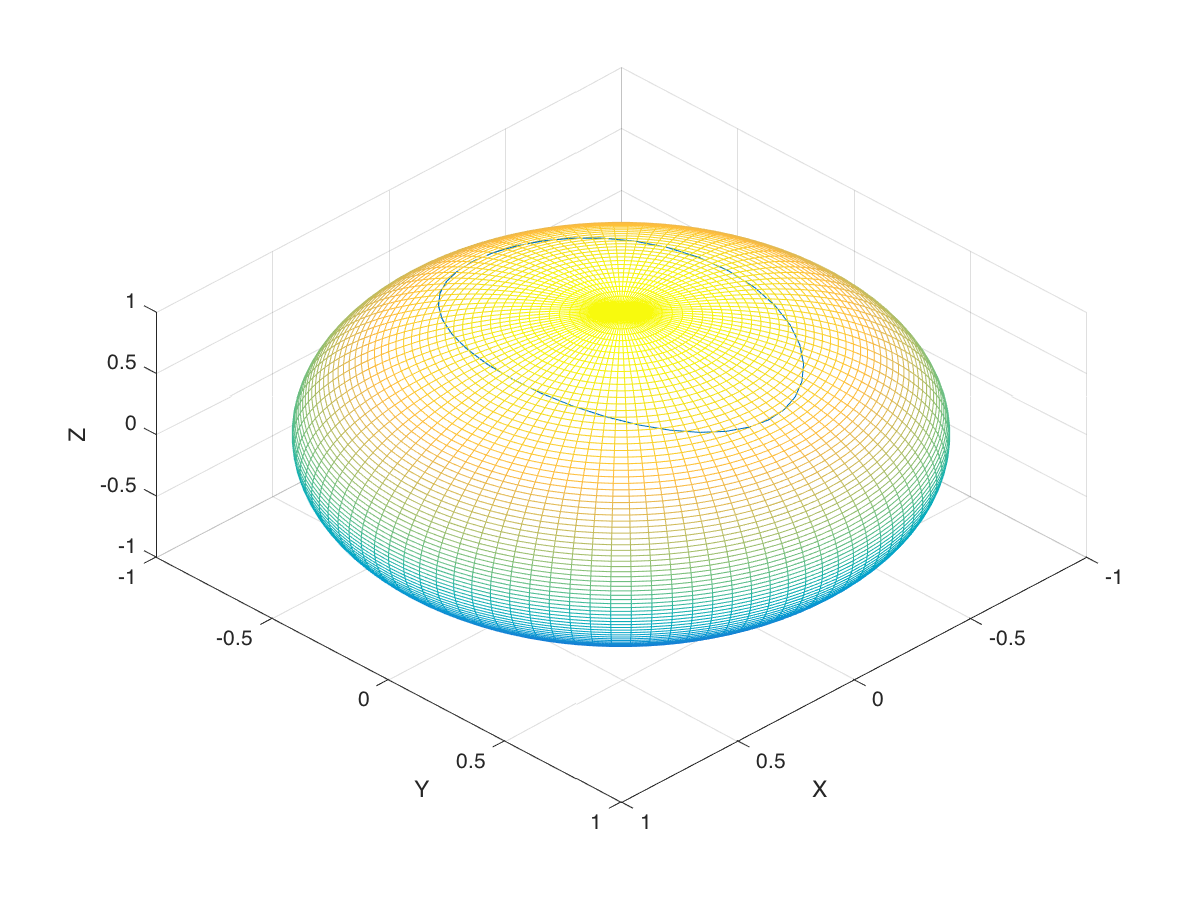
\includegraphics[width=0.6\textwidth]{03/rkmk3.png}
  \caption{改进后方法的数值结果}
  \label{fig:rkmk3}
\end{figure}

 \section{小结}\label{sec:03conclusion}
 \esection{Brief Summary}
在本章中,我们首先提出了求解哈密尔顿系统的辛波形松弛方法.该方法给出了针对该系统应该如何选择分裂函数问题的一个可行性建议.为了加速算法,使用了窗口加速技术.我们从连续系统和离散系统两个方面给出了系统哈密尔顿量在迭代下收敛到守恒的量的性质,并在数值结果中验证了这一点.

其次,在此基础上,我们对李群方法做出了详细地介绍,分析了其优点和不足,并对隐式的 RK-MK 方法提出了一种改进方法,即用波形松弛方法进行修正.该方法能够缓解隐式 RK-MK 方法的复杂性计算问题,把隐式的计算化为较为简单的显式或者半隐式问题,并用窗口技术进行加速.

最后,我们通过数值结果能够说明该方法的有效性.
